\documentclass[crop=false,class=book,oneside]{standalone}
%----------------------------Preamble-------------------------------%
%---------------------------Packages----------------------------%
\usepackage{geometry}
\geometry{b5paper, margin=1.0in}
\usepackage[T1]{fontenc}
\usepackage{graphicx, float}            % Graphics/Images.
\usepackage{natbib}                     % For bibliographies.
\bibliographystyle{agsm}                % Bibliography style.
\usepackage[french, english]{babel}     % Language typesetting.
\usepackage[dvipsnames]{xcolor}         % Color names.
\usepackage{listings}                   % Verbatim-Like Tools.
\usepackage{mathtools, esint, mathrsfs} % amsmath and integrals.
\usepackage{amsthm, amsfonts, amssymb}  % Fonts and theorems.
\usepackage{tcolorbox}                  % Frames around theorems.
\usepackage{upgreek}                    % Non-Italic Greek.
\usepackage{fmtcount, etoolbox}         % For the \book{} command.
\usepackage[newparttoc]{titlesec}       % Formatting chapter, etc.
\usepackage{titletoc}                   % Allows \book in toc.
\usepackage[nottoc]{tocbibind}          % Bibliography in toc.
\usepackage[titles]{tocloft}            % ToC formatting.
\usepackage{pgfplots, tikz}             % Drawing/graphing tools.
\usepackage{imakeidx}                   % Used for index.
\usetikzlibrary{
    calc,                   % Calculating right angles and more.
    angles,                 % Drawing angles within triangles.
    arrows.meta,            % Latex and Stealth arrows.
    quotes,                 % Adding labels to angles.
    positioning,            % Relative positioning of nodes.
    decorations.markings,   % Adding arrows in the middle of a line.
    patterns,
    arrows
}                                       % Libraries for tikz.
\pgfplotsset{compat=1.9}                % Version of pgfplots.
\usepackage[font=scriptsize,
            labelformat=simple,
            labelsep=colon]{subcaption} % Subfigure captions.
\usepackage[font={scriptsize},
            hypcap=true,
            labelsep=colon]{caption}    % Figure captions.
\usepackage[pdftex,
            pdfauthor={Ryan Maguire},
            pdftitle={Mathematics and Physics},
            pdfsubject={Mathematics, Physics, Science},
            pdfkeywords={Mathematics, Physics, Computer Science, Biology},
            pdfproducer={LaTeX},
            pdfcreator={pdflatex}]{hyperref}
\hypersetup{
    colorlinks=true,
    linkcolor=blue,
    filecolor=magenta,
    urlcolor=Cerulean,
    citecolor=SkyBlue
}                           % Colors for hyperref.
\usepackage[toc,acronym,nogroupskip,nopostdot]{glossaries}
\usepackage{glossary-mcols}
%------------------------Theorem Styles-------------------------%
\theoremstyle{plain}
\newtheorem{theorem}{Theorem}[section]

% Define theorem style for default spacing and normal font.
\newtheoremstyle{normal}
    {\topsep}               % Amount of space above the theorem.
    {\topsep}               % Amount of space below the theorem.
    {}                      % Font used for body of theorem.
    {}                      % Measure of space to indent.
    {\bfseries}             % Font of the header of the theorem.
    {}                      % Punctuation between head and body.
    {.5em}                  % Space after theorem head.
    {}

% Italic header environment.
\newtheoremstyle{thmit}{\topsep}{\topsep}{}{}{\itshape}{}{0.5em}{}

% Define environments with italic headers.
\theoremstyle{thmit}
\newtheorem*{solution}{Solution}

% Define default environments.
\theoremstyle{normal}
\newtheorem{example}{Example}[section]
\newtheorem{definition}{Definition}[section]
\newtheorem{problem}{Problem}[section]

% Define framed environment.
\tcbuselibrary{most}
\newtcbtheorem[use counter*=theorem]{ftheorem}{Theorem}{%
    before=\par\vspace{2ex},
    boxsep=0.5\topsep,
    after=\par\vspace{2ex},
    colback=green!5,
    colframe=green!35!black,
    fonttitle=\bfseries\upshape%
}{thm}

\newtcbtheorem[auto counter, number within=section]{faxiom}{Axiom}{%
    before=\par\vspace{2ex},
    boxsep=0.5\topsep,
    after=\par\vspace{2ex},
    colback=Apricot!5,
    colframe=Apricot!35!black,
    fonttitle=\bfseries\upshape%
}{ax}

\newtcbtheorem[use counter*=definition]{fdefinition}{Definition}{%
    before=\par\vspace{2ex},
    boxsep=0.5\topsep,
    after=\par\vspace{2ex},
    colback=blue!5!white,
    colframe=blue!75!black,
    fonttitle=\bfseries\upshape%
}{def}

\newtcbtheorem[use counter*=example]{fexample}{Example}{%
    before=\par\vspace{2ex},
    boxsep=0.5\topsep,
    after=\par\vspace{2ex},
    colback=red!5!white,
    colframe=red!75!black,
    fonttitle=\bfseries\upshape%
}{ex}

\newtcbtheorem[auto counter, number within=section]{fnotation}{Notation}{%
    before=\par\vspace{2ex},
    boxsep=0.5\topsep,
    after=\par\vspace{2ex},
    colback=SeaGreen!5!white,
    colframe=SeaGreen!75!black,
    fonttitle=\bfseries\upshape%
}{not}

\newtcbtheorem[use counter*=remark]{fremark}{Remark}{%
    fonttitle=\bfseries\upshape,
    colback=Goldenrod!5!white,
    colframe=Goldenrod!75!black}{ex}

\newenvironment{bproof}{\textit{Proof.}}{\hfill$\square$}
\tcolorboxenvironment{bproof}{%
    blanker,
    breakable,
    left=3mm,
    before skip=5pt,
    after skip=10pt,
    borderline west={0.6mm}{0pt}{green!80!black}
}

\AtEndEnvironment{lexample}{$\hfill\textcolor{red}{\blacksquare}$}
\newtcbtheorem[use counter*=example]{lexample}{Example}{%
    empty,
    title={Example~\theexample},
    boxed title style={%
        empty,
        size=minimal,
        toprule=2pt,
        top=0.5\topsep,
    },
    coltitle=red,
    fonttitle=\bfseries,
    parbox=false,
    boxsep=0pt,
    before=\par\vspace{2ex},
    left=0pt,
    right=0pt,
    top=3ex,
    bottom=1ex,
    before=\par\vspace{2ex},
    after=\par\vspace{2ex},
    breakable,
    pad at break*=0mm,
    vfill before first,
    overlay unbroken={%
        \draw[red, line width=2pt]
            ([yshift=-1.2ex]title.south-|frame.west) to
            ([yshift=-1.2ex]title.south-|frame.east);
        },
    overlay first={%
        \draw[red, line width=2pt]
            ([yshift=-1.2ex]title.south-|frame.west) to
            ([yshift=-1.2ex]title.south-|frame.east);
    },
}{ex}

\AtEndEnvironment{ldefinition}{$\hfill\textcolor{Blue}{\blacksquare}$}
\newtcbtheorem[use counter*=definition]{ldefinition}{Definition}{%
    empty,
    title={Definition~\thedefinition:~{#1}},
    boxed title style={%
        empty,
        size=minimal,
        toprule=2pt,
        top=0.5\topsep,
    },
    coltitle=Blue,
    fonttitle=\bfseries,
    parbox=false,
    boxsep=0pt,
    before=\par\vspace{2ex},
    left=0pt,
    right=0pt,
    top=3ex,
    bottom=0pt,
    before=\par\vspace{2ex},
    after=\par\vspace{1ex},
    breakable,
    pad at break*=0mm,
    vfill before first,
    overlay unbroken={%
        \draw[Blue, line width=2pt]
            ([yshift=-1.2ex]title.south-|frame.west) to
            ([yshift=-1.2ex]title.south-|frame.east);
        },
    overlay first={%
        \draw[Blue, line width=2pt]
            ([yshift=-1.2ex]title.south-|frame.west) to
            ([yshift=-1.2ex]title.south-|frame.east);
    },
}{def}

\AtEndEnvironment{ltheorem}{$\hfill\textcolor{Green}{\blacksquare}$}
\newtcbtheorem[use counter*=theorem]{ltheorem}{Theorem}{%
    empty,
    title={Theorem~\thetheorem:~{#1}},
    boxed title style={%
        empty,
        size=minimal,
        toprule=2pt,
        top=0.5\topsep,
    },
    coltitle=Green,
    fonttitle=\bfseries,
    parbox=false,
    boxsep=0pt,
    before=\par\vspace{2ex},
    left=0pt,
    right=0pt,
    top=3ex,
    bottom=-1.5ex,
    breakable,
    pad at break*=0mm,
    vfill before first,
    overlay unbroken={%
        \draw[Green, line width=2pt]
            ([yshift=-1.2ex]title.south-|frame.west) to
            ([yshift=-1.2ex]title.south-|frame.east);},
    overlay first={%
        \draw[Green, line width=2pt]
            ([yshift=-1.2ex]title.south-|frame.west) to
            ([yshift=-1.2ex]title.south-|frame.east);
    }
}{thm}

%--------------------Declared Math Operators--------------------%
\DeclareMathOperator{\adjoint}{adj}         % Adjoint.
\DeclareMathOperator{\Card}{Card}           % Cardinality.
\DeclareMathOperator{\curl}{curl}           % Curl.
\DeclareMathOperator{\diam}{diam}           % Diameter.
\DeclareMathOperator{\dist}{dist}           % Distance.
\DeclareMathOperator{\Div}{div}             % Divergence.
\DeclareMathOperator{\Erf}{Erf}             % Error Function.
\DeclareMathOperator{\Erfc}{Erfc}           % Complementary Error Function.
\DeclareMathOperator{\Ext}{Ext}             % Exterior.
\DeclareMathOperator{\GCD}{GCD}             % Greatest common denominator.
\DeclareMathOperator{\grad}{grad}           % Gradient
\DeclareMathOperator{\Ima}{Im}              % Image.
\DeclareMathOperator{\Int}{Int}             % Interior.
\DeclareMathOperator{\LC}{LC}               % Leading coefficient.
\DeclareMathOperator{\LCM}{LCM}             % Least common multiple.
\DeclareMathOperator{\LM}{LM}               % Leading monomial.
\DeclareMathOperator{\LT}{LT}               % Leading term.
\DeclareMathOperator{\Mod}{mod}             % Modulus.
\DeclareMathOperator{\Mon}{Mon}             % Monomial.
\DeclareMathOperator{\multideg}{mutlideg}   % Multi-Degree (Graphs).
\DeclareMathOperator{\nul}{nul}             % Null space of operator.
\DeclareMathOperator{\Ord}{Ord}             % Ordinal of ordered set.
\DeclareMathOperator{\Prin}{Prin}           % Principal value.
\DeclareMathOperator{\proj}{proj}           % Projection.
\DeclareMathOperator{\Refl}{Refl}           % Reflection operator.
\DeclareMathOperator{\rk}{rk}               % Rank of operator.
\DeclareMathOperator{\sgn}{sgn}             % Sign of a number.
\DeclareMathOperator{\sinc}{sinc}           % Sinc function.
\DeclareMathOperator{\Span}{Span}           % Span of a set.
\DeclareMathOperator{\Spec}{Spec}           % Spectrum.
\DeclareMathOperator{\supp}{supp}           % Support
\DeclareMathOperator{\Tr}{Tr}               % Trace of matrix.
%--------------------Declared Math Symbols--------------------%
\DeclareMathSymbol{\minus}{\mathbin}{AMSa}{"39} % Unary minus sign.
%------------------------New Commands---------------------------%
\DeclarePairedDelimiter\norm{\lVert}{\rVert}
\DeclarePairedDelimiter\ceil{\lceil}{\rceil}
\DeclarePairedDelimiter\floor{\lfloor}{\rfloor}
\newcommand*\diff{\mathop{}\!\mathrm{d}}
\newcommand*\Diff[1]{\mathop{}\!\mathrm{d^#1}}
\renewcommand*{\glstextformat}[1]{\textcolor{RoyalBlue}{#1}}
\renewcommand{\glsnamefont}[1]{\textbf{#1}}
\renewcommand\labelitemii{$\circ$}
\renewcommand\thesubfigure{%
    \arabic{chapter}.\arabic{figure}.\arabic{subfigure}}
\addto\captionsenglish{\renewcommand{\figurename}{Fig.}}
\numberwithin{equation}{section}

\renewcommand{\vector}[1]{\boldsymbol{\mathrm{#1}}}

\newcommand{\uvector}[1]{\boldsymbol{\hat{\mathrm{#1}}}}
\newcommand{\topspace}[2][]{(#2,\tau_{#1})}
\newcommand{\measurespace}[2][]{(#2,\varSigma_{#1},\mu_{#1})}
\newcommand{\measurablespace}[2][]{(#2,\varSigma_{#1})}
\newcommand{\manifold}[2][]{(#2,\tau_{#1},\mathcal{A}_{#1})}
\newcommand{\tanspace}[2]{T_{#1}{#2}}
\newcommand{\cotanspace}[2]{T_{#1}^{*}{#2}}
\newcommand{\Ckspace}[3][\mathbb{R}]{C^{#2}(#3,#1)}
\newcommand{\funcspace}[2][\mathbb{R}]{\mathcal{F}(#2,#1)}
\newcommand{\smoothvecf}[1]{\mathfrak{X}(#1)}
\newcommand{\smoothonef}[1]{\mathfrak{X}^{*}(#1)}
\newcommand{\bracket}[2]{[#1,#2]}

%------------------------Book Command---------------------------%
\makeatletter
\renewcommand\@pnumwidth{1cm}
\newcounter{book}
\renewcommand\thebook{\@Roman\c@book}
\newcommand\book{%
    \if@openright
        \cleardoublepage
    \else
        \clearpage
    \fi
    \thispagestyle{plain}%
    \if@twocolumn
        \onecolumn
        \@tempswatrue
    \else
        \@tempswafalse
    \fi
    \null\vfil
    \secdef\@book\@sbook
}
\def\@book[#1]#2{%
    \refstepcounter{book}
    \addcontentsline{toc}{book}{\bookname\ \thebook:\hspace{1em}#1}
    \markboth{}{}
    {\centering
     \interlinepenalty\@M
     \normalfont
     \huge\bfseries\bookname\nobreakspace\thebook
     \par
     \vskip 20\p@
     \Huge\bfseries#2\par}%
    \@endbook}
\def\@sbook#1{%
    {\centering
     \interlinepenalty \@M
     \normalfont
     \Huge\bfseries#1\par}%
    \@endbook}
\def\@endbook{
    \vfil\newpage
        \if@twoside
            \if@openright
                \null
                \thispagestyle{empty}%
                \newpage
            \fi
        \fi
        \if@tempswa
            \twocolumn
        \fi
}
\newcommand*\l@book[2]{%
    \ifnum\c@tocdepth >-3\relax
        \addpenalty{-\@highpenalty}%
        \addvspace{2.25em\@plus\p@}%
        \setlength\@tempdima{3em}%
        \begingroup
            \parindent\z@\rightskip\@pnumwidth
            \parfillskip -\@pnumwidth
            {
                \leavevmode
                \Large\bfseries#1\hfill\hb@xt@\@pnumwidth{\hss#2}
            }
            \par
            \nobreak
            \global\@nobreaktrue
            \everypar{\global\@nobreakfalse\everypar{}}%
        \endgroup
    \fi}
\newcommand\bookname{Book}
\renewcommand{\thebook}{\texorpdfstring{\Numberstring{book}}{book}}
\providecommand*{\toclevel@book}{-2}
\makeatother
\titleformat{\part}[display]
    {\Large\bfseries}
    {\partname\nobreakspace\thepart}
    {0mm}
    {\Huge\bfseries}
\titlecontents{part}[0pt]
    {\large\bfseries}
    {\partname\ \thecontentslabel: \quad}
    {}
    {\hfill\contentspage}
\titlecontents{chapter}[0pt]
    {\bfseries}
    {\chaptername\ \thecontentslabel:\quad}
    {}
    {\hfill\contentspage}
\newglossarystyle{longpara}{%
    \setglossarystyle{long}%
    \renewenvironment{theglossary}{%
        \begin{longtable}[l]{{p{0.25\hsize}p{0.65\hsize}}}
    }{\end{longtable}}%
    \renewcommand{\glossentry}[2]{%
        \glstarget{##1}{\glossentryname{##1}}%
        &\glossentrydesc{##1}{~##2.}
        \tabularnewline%
        \tabularnewline
    }%
}
\newglossary[not-glg]{notation}{not-gls}{not-glo}{Notation}
\newcommand*{\newnotation}[4][]{%
    \newglossaryentry{#2}{type=notation, name={\textbf{#3}, },
                          text={#4}, description={#4},#1}%
}
%--------------------------LENGTHS------------------------------%
% Spacings for the Table of Contents.
\addtolength{\cftsecnumwidth}{1ex}
\addtolength{\cftsubsecindent}{1ex}
\addtolength{\cftsubsecnumwidth}{1ex}
\addtolength{\cftfignumwidth}{1ex}
\addtolength{\cfttabnumwidth}{1ex}

% Indent and paragraph spacing.
\setlength{\parindent}{0em}
\setlength{\parskip}{0em}                                                %
\graphicspath{{images/}}   % Path to Image Folder.                  %
%----------------------------GLOSSARY-------------------------------%
\makeglossaries                                                     %
\loadglsentries{glossary}                                           %
\loadglsentries{acronym}                                            %
%--------------------------Main Document----------------------------%
\begin{document}
    \ifx\ifmathcourses\undefined
        \pagenumbering{roman}
        \title{Convex Geometry}
        \author{Ryan Maguire}
        \date{\vspace{-5ex}}
        \maketitle
        \tableofcontents
        \clearpage
        \chapter{Convex Geometry}
        \setcounter{chapter}{1}
        \pagenumbering{arabic}
    \else
        \chapter{Convex Geometry}
    \fi
    \section{Convexity: Part I}
        \subsection{Convex Sets}
            \begin{definition}
            A subset $K$ of a Banach Space $X$ is convex if and only if $\big[[x,y\in K]\land  [\lambda \in [0,1]]\big]\Rightarrow[(1-\lambda)x+\lambda y\in K]$.
            \end{definition}
            \begin{theorem}
            Convex spaces are path-connected.
            \end{theorem}
            \begin{proof}
            Let $x,y\in V$ and define $f:[0,1]\rightarrow V$ by $f(\lambda) = (1-\lambda)x+\lambda y$. Therefore, etc.
            \end{proof}
            \begin{corollary}
            Convex sets are connected.
            \end{corollary}
            \begin{proof}
            As convex sets are path-connected, they are connected.
            \end{proof}
            \begin{theorem}
            Any Banach Space $X$ is convex.
            \end{theorem}
            \begin{proof}
            Let $x,y\in V$. As $V$ is a vector space, for all $\lambda \in \mathbb{R}$, $(1-\lambda)x+\lambda y\in V$. Therefore, etc.
            \end{proof}
            \begin{notation}
            The set of all convex subsets of $\mathbb{R}^n$ is denoted $\mathscr{K}_n$.
            \end{notation}
            \begin{theorem}
            If $X$ is a Banach Space and $A,B\subset X$ are convex sets, then $A\cap B$ is convex.
            \end{theorem}
            \begin{proof}
            $[x,y \in A\cap B] \Rightarrow \big[[\lambda \in [0,1]]\Rightarrow[ (1-\lambda)x+\lambda y \in A]\land [ (1-\lambda)x+\lambda y \in B]\big] \Rightarrow [\forall \lambda \in [0,1]:(1-\lambda)x+\lambda y \in A\cap B]$. 
            \end{proof}
            \begin{lemma}
            In a Banach Space $X$, $\forall \xi \in X$, $\forall r>0$, $B_{r}(\xi)$ is convex.
            \end{lemma}
            \begin{proof}
            $[x,y\in B_{r}(\xi)]\Rightarrow\big[[\lambda \in [0,1]]\Rightarrow [\norm{(1-\lambda)x+\lambda y-\xi}\leq \frac{(1-\lambda)}{2}\norm{x-\xi}+\frac{\lambda}{2} \norm{y-\xi}< r]\big]\Rightarrow [(1-\lambda)x+\lambda y \in B_{r}(\xi)]$.
            \end{proof}
            \begin{theorem}
            There exist convex sets $A$ and $B$ such that $A\cap B \ne \emptyset$, yet $A\cup B$ is not convex.
            \end{theorem}
            \begin{proof}
            For let $A = \{(x,y)\in \mathbb{R}^2: (x-1)^2+y^2\leq 1\}$, and $B = \{(x,y)\in \mathbb{R}^2:(x+1)^2+y^2\leq 1\}$. Both of these sets are discs, and thus convex, their intersection is the point $(0,0)$, however their union is not convex.
            \end{proof}
            \begin{theorem}
            If $K\subset X$ is convex and $\psi:X\rightarrow X$ is a linear transformation, then $\psi(K)$ is convex.
            \end{theorem}
            \begin{proof}
            $[X,Y\in \psi(K)]\Rightarrow [\exists x,y\in K:\psi(x)=X\land \psi(y)=Y]$. $\big[\lambda \in [0,1]\big]\Rightarrow [(1-\lambda)x+\lambda y\in K]\Rightarrow [\psi\big((1-\lambda)x+\lambda y\big)=(1-\lambda)\psi(x)+\lambda\psi(y) = (1-\lambda)X+\lambda Y \in \psi(K)]$
            \end{proof}
            \begin{theorem}
            There exist non-convex, compact subsets $K$ of a Banach Space $X: K_{\xi}$ is convex for every subspace $\xi$.
            \end{theorem}
            \begin{proof}
            Let $r>0, \mathcal{M} = \{B_{r}(\mathbf{0})\setminus B_{r/2}(\mathbf{0})\}$. This is not convex, but for any subspace $\xi$, $\mathcal{M}_{\xi} = B_{r}(\mathbf{0})\cap \xi$, which is convex.
            \end{proof}
            \begin{theorem}
            If $X$ is a Banach Space, $K\subset X$, and for every affine subspace $\xi$, $K\cap \xi$ is convex, then $K$ is convex.
            \end{theorem}
            \begin{proof}
            Let $x,y\in K$. Let $W$ be a subspace containing $y$, and let $\xi$ be the affine subspace $\{x-y+v:v\in W\}$. Then $\xi\cap K$ is convex, and thus $(1-\lambda)x+\lambda y \in \xi \cap K \Rightarrow (1-\lambda)x+\lambda y \in K$.
            \end{proof}
            \begin{theorem}
            If $X$ is a Banach Space, $K,L\subset X$ are convex, then $K+L$ is convex.
            \end{theorem}
            \begin{proof}
            For let $\chi$ and $\zeta$ be elements of $K+L$. Then there are points $x_1,x_2$ and $y_1,y_2$ such that $\chi=x_1+x_2$ and $\zeta = y_1+y_2$ with $x_1,y_1\in K$ and $x_2,y_2\in L$. If $\lambda \in [0,1]$, then $(1-\lambda)\chi + \lambda \zeta = (1-\lambda)(x_1+x_2)+\lambda(y_1+y_2) = (1-\lambda)x_1 + \lambda y_1 + (1-\lambda)x_2 + \lambda y_2$. But $K$ and $L$ are convex, and thus $(1-\lambda)x_1 + \lambda y_1 \in K$ and $(1-\lambda)x_2 + \lambda y_2 \in L$. But then $(1-\lambda)x_1 + \lambda y_1 + (1-\lambda)x_2 + \lambda y_2=(1-\lambda)\chi + \lambda \zeta\in K+L$. As $\lambda$ is arbitrary in $[0,1]$, $K+L$ is convex.
            \end{proof}
            \begin{theorem}
            If $V$ is a Banach Space, $K\subset V$ is convex, and $\alpha \in \mathbb{R}$, then $\alpha K$ is convex.
            \end{theorem}
            \begin{proof}
            For let $X,Y\in \alpha K$. Then $X = \alpha x$ and $Y = \alpha y$ for $x,y\in K$. Let $\lambda \in (0,1)$ be arbitrary. Then $(1-\lambda)X+\lambda Y =(1-\lambda)(\alpha x)+\lambda (\alpha y) = \alpha\big[(1-\lambda)x+\lambda y\big]$. As $K$ is convex, $(1-\lambda)x+\lambda y \in K$. Thus $\alpha\big[(1-\lambda)x+\lambda y\big] \in \alpha K$, and $\alpha K$ is convex.
            \end{proof}
            \begin{theorem}
            If $K$ and $L$ are compact and convex, and $K\cup L$ is convex, then $K\cap L \ne \emptyset$.
            \end{theorem}
            \begin{proof}
            For if not, then $K\cup L$ is the union of two closed, disjoint subsets, and is thus disconnected. A contradiction. 
            \end{proof}
            \begin{lemma}
            Any set is a subset of its convex hull.
            \end{lemma}
            \begin{proof}
            For $x\in K \Rightarrow 1\cdot x=x \in \textrm{conv}(K)$. Therefore, etc.
            \end{proof}
            \begin{lemma}
            If $x\in \textrm{conv}(K)$, then there are two points in $\textrm{conv}(K)$ such that $x = \lambda v_1 +(1- \lambda) v_2$, $0 \leq \lambda \leq 1$.
            \end{lemma}
            \begin{proof}
            Let $x=\sum_{k=1}^{n+1}|\lambda_k| x_k$. If $x=|\lambda_{n+1}|x_{n+1}$, we are done. If not, then let $v_2 = \frac{1}{1-|\lambda_{n+1}|}\sum_{k=1}^{n}|\lambda_k|x_k$. As $\frac{1}{1-|\lambda_{n+1}|}\sum_{k=1}^{n}|\lambda_k| = 1$, $v_1\in \textrm{conv}(K)$. Thus, $x = \lambda_{n+1}x_{n+1}+(1-\lambda_{n+1})v_2$. Let $x_{n+1}=v_1$ and $\lambda = \lambda_{n+1}$. Therefore, etc.
            \end{proof}
            \begin{theorem}
            The convex hull of a convex set is itself.
            \end{theorem}
            \begin{proof}
            $[x\in \textrm{conv}(K)]\Rightarrow [\exists v_1,v_2\in K\land \lambda\in[0,1]:x=\lambda v_1+(1-\lambda)v_2]\Rightarrow [x\in K]$. The last step is from convexity.
            \end{proof}
            \begin{theorem}
            If $K$ is compact and convex, $\lambda_n\in[0,1]$, $v_n\in K$, and $\sum_{k=1}^{n}\lambda_k \rightarrow 1$, then $\sum_{k=1}^{n}\lambda_k v_k$ converges in $K$.
            \end{theorem}
            \begin{proof}
            Let $x\in K$ be arbitrary, $\varepsilon>0$, $s_n = \sum_{k=1}^{n}\lambda_k v_k$, and $\Lambda_n = \sum_{k=1}^{n}\lambda_k$. Let $S_n = s_n + (1-\Lambda_n)x$. For each $n\in \mathbb{N}$, $S_n\in K$. It now suffices to show $S_n$ converges. As $K$ is compact, $\{\norm{v}:v\in K\}$ is bounded, let $M$ be a bound. As $\Lambda_n\rightarrow 1$, $\exists N\in \mathbb{N}:n,m>N\Rightarrow |\Lambda_n-\Lambda_m|<\frac{\varepsilon}{2M}$. But then for $n\geq m >N$, $d(S_n,S_m) = \norm{\sum_{k=m}^{n}\lambda_k v_k+x(\Lambda_n-\Lambda_m)} \leq \sum_{k=m}^{n}|\lambda_k| \norm{v_k}+\norm{x}|(\Lambda_n-\Lambda_m)|\leq 2M|\Lambda_{n}-\Lambda_{m}|<\varepsilon$. Thus, $S_n$ is Cauchy. As $K$ is compact, it is complete, and thus $S_n$ converges in $K$. But $d(S_n,s_n)\leq |1-\Lambda_n|M\rightarrow 0$. Thus, $s_n$ converges to the same limit. Therefore, etc.
            \end{proof}
            \begin{theorem}
            The convex hull of a compact set is compact.
            \end{theorem}
            \begin{proof}
            Yeah
            \end{proof}
            \begin{theorem}
            The convex hull of an open set is open.
            \end{theorem}
            \begin{proof}
            Let $x\in \textrm{conv}(K)$. Then $x=\sum_{k=1}^{n}|\lambda_k| x_k$, where $\sum_{k=1}^{n}|\lambda_k| = 1$. At least one $\lambda_k$ must be non-zero, suppose $\lambda_1$ is. Define the function $f:\textrm{K}\rightarrow \textrm{K}$ by $f(z) = \frac{1}{|\lambda_1|}(z-\sum_{k=2}^{n}|\lambda_k|v_k$. Then $f$ is continuous, injective, and thus $f^{-1}$ exists and is equal to $f^{-1}(z) = \lambda_1 z +\sum_{k=2}^{n}\lambda_k v_k$. Thus, $x\in f^{-1}(K)\subset\textrm{conv}(K)$. Therefore, etc. 
            \end{proof}
            \begin{theorem}
            There exist closed sets whose convex hull is open (And not closed).
            \end{theorem}
            \begin{proof}
            Let $K = \{(x,y)\in \mathbb{R}^2:\frac{1}{1+x^2}\leq y\}$. The complement is open, and thus this is closed. But $\textrm{conv}(K) = \{(x,y)\in \mathbb{R}^2:y>0\}$, which is open. As $\mathbb{R}^2$ is connected, this set is not closed.
            \end{proof}
            \begin{theorem}[Carath\'{e}odory's Theorem]
            If $S$ is an $n$ dimensional subset of a Banach Space, there there exists $n+1$ points $x_k$ in $S$ such that $\textrm{conv}(S) = \textrm{conv}(x_1,\hdots, x_{n+1})$.
            \end{theorem}
            \begin{proof}
            Let $y\in \textrm{conv}(S)$. If $y\notin S$, then there are points $x_1,\hdots, x_m$ and positive real numbers $\lambda_1,\hdots, \lambda_m$ such that $y=\sum_{k=1}^{m}\lambda_m x_m$ and $\sum_{k=1}^{m}\lambda_k = 1$. Let $m$ be the minimal number of points needed. Suppose the $x_i$ are affinely dependent. Then there are real numbers $\alpha_i$ such that $\sum_{k=1}^{m}\alpha_k x_k = \mathbf{0}$ and $\sum_{k=1}^{n}\alpha_k =1$. But then $y = y+t\mathbf{0}$ for all $t\in \mathbb{R}$, and thus $y = \sum_{k=1}^{m}\lambda_k x_k + t\sum_{k=1}^{m}\alpha_k x_k = \sum_{k=1}^{m}(\lambda_k + t\alpha_k)x_k$ and $\sum_{k=1}^{m}(\lambda_k+t\alpha_t) = 1$. Let $|t|$ be the smallest value such that $\lambda_j + t\alpha_j = 0$ for some $j$. Then, for all other values, $\lambda_k + t\alpha_k \in [0,1]$. Thus, $y$ is represented by a convex combination of $m-1$ points, a contradiction as $m$ is minimal. Thus, the $x_k$ are affinely independent. But then $m \leq n+1$. Thus, etc.
            \end{proof}
            \begin{definition}
            A set $P$ is said to be a convex polytope if and only if it is the convex hull of finitely many points.
            \end{definition}
            \begin{definition}
            A polytope in $\mathbb{R}^2$ is called a polygon.
            \end{definition}
            \begin{notation}
            The set of all polytopes in $\mathbb{R}^n$ is denoted $\mathscr{P}_n$.
            \end{notation}
            \begin{definition}
            A polytope $P$ is said to be a simplex if and only if then generating points are affinely independent.
            \end{definition}
            \begin{theorem}
            An $n$ dimensional simplex has $n+1$ vertices.
            \end{theorem}
            \begin{theorem}
            If $P$ is a polytope in some Banach Space $V$, and $\xi$ is a subspace, then $P_{\xi}$ is a polytope.
            \end{theorem}
            \begin{theorem}
            If $K$ is a compact set of finite dimension $n\geq 3$, and if for every $n-1$ dimensional subspace $\xi$, $K_{\xi}$ is a convex polytope, then $K$ is a convex polytope. (Page 23)
            \end{theorem}
            \begin{theorem}[Radon's Theorem]
            If $S$ Is a finite dimensional affinely dependent subset of a Banach Space $V$, then there are sets $S_1,S_2\in V$ such that $S_1\cap S_2 = \emptyset$, $S=S_1\cup S_2$, and $\textrm{conv}(S_1)\cap \textrm{conv}(S_2) \ne \emptyset$.
            \end{theorem}
            \begin{proof}
            As $S$ is affinely dependent, there are distinct points $x_1,\hdots,x_n$ and non-zero real numbers $\lambda_1,\hdots,\lambda_n$ such that $\sum_{k=1}^{n}\lambda_k x_k= \mathbf{0}$ and $\sum_{k=1}^{n}\lambda_k = 0$. As none of the values of $\lambda_k$ are zero, some most be positive and some negative. Let $\lambda_1,\hdots, \lambda_j$ be positive and $\lambda_{j+1},\hdots, \lambda_n$ are negative. Then $\sum_{k=1}^{j} \lambda_k = - \lambda_{k=j+1}^{n}\lambda_k$. Let this sum be $c$. Let $T_1 = \{x_1,\hdots, x_j\}$ and $T_2=\{x_{j+1},\hdots, x_{n}\}$. As the $x_k$ are distinct, $T_1\cap T_2 = \emptyset$. However, $\frac{1}{c}\sum_{k=1}^{j}\lambda_k x_k = \frac{-1}{c}\sum_{k=j+1}^{n} \lambda_k x_k \in\textrm{conv}(T_1)\cap \textrm{conv}(T_2)$. Let $S_1 = S\setminus T_2$, and $S_2 = T_2$. Therefore, etc.
            \end{proof}
            \begin{theorem}
            If $K$ is compact, convex, and a subset of a two dimensional Banach Space, then if $A = \{x\in K:B_{1}(x)\subset K\}$, then $\underset{x\in A}\cup B_{1}(x)$ is convex.
            \end{theorem}
            \begin{theorem}
            If $K$ is a compact, convex subset of a two dimensional Banach Space, then $\underset{x\in K}\cup B_{1}(x)$ is convex.
            \end{theorem}
        \subsection{Convexity in the Euclidean Plane}
            \begin{definition}
            $A(K)$ is the area of a compact set $K$.
            \end{definition}
            \begin{definition}
            The perimeter $P(K)$ is the length of the boundary curve, $\mu(\partial K)$.
            \end{definition}
            \begin{definition}
            The section $X_{\ell}(K)$ is defined for any given straight line $\ell$ to be the length $\mu(K\cap \ell)$.
            \end{definition}
            \begin{definition}
            Given a straight line $\ell$, the width $W_{\ell}(K)$ is $\mu(\ell_{K})$.
            \end{definition}
            \begin{definition}
            The mean width $W(K)$ is the average of the width of all $W_{\ell}(K)$.
            \end{definition}
            \begin{definition}
            The minimum width $w(K)$ is the minimum of $W_{\ell}(K)$ over all possible directions of the line $\ell$.
            \end{definition}
            \begin{definition}
            The maximum width $\check{W}$ is the maximum of $W_{\ell}(K)$.
            \end{definition}
            \begin{definition}
            The diameter $D(K)$ is the maximum distance between any two points inside $K$.
            \end{definition}
            \begin{definition}
            The inradius $r_K$ is the maximum radius of any circle inside $K$.
            \end{definition}
            \begin{definition}
            The circumradius $R_K$ is the minimum radius of any circle containing $K$.
            \end{definition}
            \begin{notation}
            For bounded sets $K\subset \mathbb{R}^2$, define $R_K(\theta)$ as the projection or $K$ onto the line $\sin(\theta)y=\cos(\theta)x$.
            \end{notation}
            \begin{theorem}
            If $K$ is a compact subset of $\mathbb{R}^n$, then there are points $x,y\in K$ such that $d(x,y)=D(K)$.
            \end{theorem}
            \begin{proof}
            As $K$ is compact, it is bounded. Let $M$ be such a bound. Then the set $D=\{r\in \mathbb{R}^+| d(x,y) = r,\ x,y\in K\}$ is bounded by $M$. Let $d$ be the least upper bound of this set. Then we can find a sequence of points $x_n,y_n\in K$ such that $d(x_n,y_n) \rightarrow d$. As $K$ is compact, there are convergent subsequence $x_{n_k}$ and $y_{n_k}$ with limits in $K$, call them $x$ and $y$. Then $d(x,y) = d$. Thus, there are points $x,y\in K$ such that $d(x,y) \geq d(a,b)$ for all $a,b\in K$. Therefore $D(K)$ is equal to $d$.
            \end{proof}
            \begin{theorem}
                \label{thm:Convex_Geo_Bounded_Set_Discon_Angle_Proj_Func}
                There exist bounded sets $K$ such that $R_K(\theta)$
                is not continuous.
            \end{theorem}
            \begin{proof}
                For define:
                \begin{equation}
                    \mathcal{M}=
                        \{(x,y)\in [-1,1]^2:
                            x\in\mathbb{Q},y\in \mathbb{R}\}
                \end{equation}
                Also, let $K=\mathcal{M}\cap\overline{D^{2}}$,
                where $\overline{D^{2}}$ denotes the closed unit
                disc in $\mathbb{R}^{2}$. Then $f_{K}(\theta)$ is
                discontinuous at $\theta=\frac{\pi}{2}$. For,
                $f_K(\frac{\pi}{2})=\mu(\mathbb{Q}\cap [-1,1])=0$. But,
                for any $0<\delta<\pi$,
                $f_K(\frac{\pi}{2}\pm\delta)=2$. Thus:
                \begin{equation}
                    f_K(\theta)=
                        \begin{cases}
                            0,&\theta=\pm\frac{\pi}{2}\\
                            2,&\theta\ne\pm\frac{\pi}{2}
                        \end{cases}
                \end{equation}
                And this is discontinuous.
            \end{proof}
            \begin{figure}[H]
                \centering
                \captionsetup{type=figure}
                %----------------------------------Preamble------------------------------------%
%   \usepackage{tikz}                   % Drawing/graphing tools.   
%       angles                          % Drawing angles within triangles.
%       quotes                          % Adding labels to angles.
%-------------------------------Main Document----------------------------------%
\begin{tikzpicture}
    \coordinate (O) at (0, 0);
    \coordinate (A) at (0, 1in);
    \coordinate (B) at (0.7071in, 0.7071in);
    \coordinate (C) at (0, 1.414in);
    \coordinate (D) at (1in, 1in);
    \coordinate (E) at (1.414in, 0);
    \draw (O) circle (1in);
    \draw (-1.1in, 1in) to (1.1in, 1in);
    \draw (O) to (0, 1.5in);
    \draw (A) to (B);
    \draw (O) to (D);
    \draw (C) to (E);
    \draw[fill=black] (O) circle (0.4mm);
    \draw[fill=black] (A) circle (0.4mm);
    \draw[fill=black] (B) circle (0.4mm);
    \draw[fill=black] (C) circle (0.4mm);
    \draw[fill=black] (D) circle (0.4mm);
    \node at (O) [below left] {$O$};
    \node at (A) [above left] {$A$};
    \node at (B) [right] {$B$};
    \node at (C) [right] {$C$};
    \node at (D) [above] {$D$};
    \pic[%
        draw=black,
        "\scriptsize{${\theta}$}",
        angle eccentricity=1.7,
        angle radius =0.5cm
    ]   {angle = D--O--C};
\end{tikzpicture}
                \caption{Drawing for Thm.~\ref{thm:Convex_Geo_Bounded_%
                    Set_Discon_Angle_Proj_Func}.}
                \label{fig:Convex_Geo_Bounded_Set_Discon_Angle_Func}
            \end{figure}
            \begin{theorem}
                \label{thm:Convex_Geo_Proj_Ang_Func_Cont_Comp_Conv}
                If $K\subset\mathbb{R}^2$ is compact and convex,
                then $R_K(\theta)$ is continuous.
            \end{theorem}
            \begin{proof}
                For let $K$ be compact and convex, and without loss
                of generality suppose it contained within the unit disc
                and contains the origin. Let $\theta\in (0,2\pi)$ be
                given and let $\ell_{\theta}$ be a line through the
                origin making an angle $\theta$ with the horizontal.
                Let $x=(x_1,x_2)$, $y=(y_1,y_2)\in{K}$ be such that
                $W_{\ell_{\theta}}(K)=d(x,y)$. Such points exist as
                $K$ is compact. Let $\varepsilon>0$ be given. About $x$,
                consider $B_{\frac{\varepsilon}{2}}(x)$, and similarly
                $B_{\frac{\varepsilon}{2}}(y)$. Neither of these are
                empty, as $K$ is convex. Let $x',y'\in K\cap(B_{\frac{\varepsilon}{2}}(x)\cup B_{\frac{\varepsilon}{2}}(y))$ be such that $d(x',y')$
                is maximized. As this set is compact, such points exist.
                Let $\delta$ be defined by:
                \begin{equation}
                    \delta=
                    \min\{|\theta-\frac{x_2'}{\sqrt{x_1'^2+x_2'^2}}|,
                        |\theta-\frac{y_2'}{\sqrt{y_1'^2+y_2'^2}}|\}
                \end{equation}
                Then, since $|\theta-\theta_0|<\delta$:
                \begin{equation}
                    d(x,y)-\varepsilon\leq
                    W_{\ell_{\theta_0}}(K)\leq
                    d(x,y)+\varepsilon
                \end{equation}
                and thus $|W_{\ell_\theta}(K)-W_{\ell_{\theta_0}}(K)|< \varepsilon$.
            \end{proof}
            \begin{figure}
                \centering
                \captionsetup{type=figure}
                %----------------------------------Preamble------------------------------------%
%   \usepackage{tikz}                   % Drawing/graphing tools.   
%       angles                          % Drawing angles within triangles.
%       quotes                          % Adding labels to angles.
%-------------------------------Main Document----------------------------------%
\begin{tikzpicture}
    \coordinate (x) at (-0.3in, -1.0in);
    \coordinate (y) at (0.5in, 0.3in);
    \coordinate (xp) at (-0.397in, -0.937in);
    \coordinate (yp) at (0.5in, 0.185in);
    \coordinate (O) at (0.2in, -0.19in);
    \node at (x) [below] {$x$};
    \node at (y) [right] {$y$};
    \node at (xp) [above] {$x'$};
    \node at (yp) [right] {$y'$};
    \pic[%
        draw=black,
        "\scriptsize{${\delta}$}",
        angle eccentricity=1.2,
        angle radius=1.2cm
    ]   {angle=xp--O--x};
    \draw (-1.0in, 0.1in)
        to [out=-90,in=150] (x)
        to [out=-30,in=-90] (0.5in,-0.75in)
        to [out=90,in=-90] (0.5in, 0.8in)
        to [out=110, in=30] (-0.5in, 0.7in)
        to (-1.0in, 0.1in);
    \draw[fill=black] (x) circle (0.3mm);
    \draw[fill=black] (y) circle (0.3mm);
    \draw[fill=black] (xp) circle (0.3mm);
    \draw[fill=black] (yp) circle (0.3mm);
    \clip (-1.0in, 0.1in)
        to [out=-90,in=150] (x)
        to [out=-30,in=-90] (0.5in,-0.75in)
        to [out=90,in=-90] (0.5in, 0.8in)
        to [out=110, in=30] (-0.5in, 0.7in)
        to (-1.0in, 0.1in);
    \draw[fill=cyan, opacity=0.3] (x) circle (3mm);
    \draw[fill=cyan, opacity=0.3] (y) circle (3mm);
    \draw[draw=blue] (x) to (y);
    \draw[draw=red] (xp) to (yp);
    \draw[fill=black] (x) circle (0.3mm);
    \draw[fill=black] (y) circle (0.3mm);
    \draw[fill=black] (xp) circle (0.3mm);
    \draw[fill=black] (yp) circle (0.3mm);
\end{tikzpicture}
                \caption{Drawing for Thm.~\ref{thm:Convex_Geo_Proj_Ang_%
                    Func_Cont_Comp_Conv}.}
                \label{fig:Convex_Geo_Proj_Ang_Func_Cont_Comp_Conv}
            \end{figure}
            \begin{theorem}
                \label{thm:Convex_Geo_Two_Lines_Which_Contain_All_Comp_Conv}
                If $K$ is a compact subset of $\mathbb{R}^2$ and
                $x,y\in{K}$ such that $d(x,y)=D(K)$, then the
                lines perpendicular to $\overline{xy}$ at $x$ and
                $y$ contain all of $K$ in between.
            \end{theorem}
            \begin{proof}
                Suppose not. Let $\overline{X}$ be the line perpendicular to
                $\overline{xy}$ containing point $x$, and similarly define
                $\overline{Y}$. Suppose there is a point $z\in K$ that falls
                on the exterior of the region:
                \begin{equation}
                    \mathcal{U}=\{(x,y)\in\mathbb{R}^{2}:
                        (x,y)\textrm{ Lies Between }\overline{X}
                        \textrm{ and }\overline{Y}\}
                \end{equation}
                Note that $d(x,z)\ne d(y,z)$, as then $z$ would line
                between these two lines. Suppose $d(y,z)<d(x,z)$. Where
                the line $\overline{xz}$ cuts $\overline{Y}$ denote as
                $A$. But then:
                \begin{equation}
                    d(x,z)>d(x,A)=
                    \sqrt{d(y,A)^2+d(x,y)^2}\geq
                    d(x,y)
                \end{equation}
                A contradiction as $d(x,y)=D(K)$. Thus $z\in\mathcal{U}$.
            \end{proof}
            \begin{figure}[H]
                \centering
                \captionsetup{type=figure}
                \documentclass[crop,class=article]{standalone}
%----------------------------Preamble-------------------------------%
\usepackage{pgfplots, tikz}             % Drawing/graphing tools.
\pgfplotsset{compat=1.9}                % Version of pgfplots.
%--------------------------Main Document----------------------------%
\begin{document}
    \begin{tikzpicture}
        \coordinate (x) at (0, 0);
        \coordinate (y) at (0, 1in);
        \coordinate (a) at (1in, 1in);
        \coordinate (z) at (1.3in, 1.3in);
        \draw[thick] (-1in, 0) to (1.5in, 0);
        \draw[thick] (-1in, 1in) to (1.5in, 1in);
        \draw[thick] (x) to (y);
        \draw[thick] (x) to (z);
        \draw[decorate, decoration={brace,amplitude=6pt}]
            (x) to node [xshift=-0.9cm] {$d(x,y)$} (y);
        \draw[decorate, decoration={brace,amplitude=6pt}]
            (a) to node [xshift=0.7cm,yshift=-0.5cm] {$d(x,a)$} (x);
        \draw[decorate, decoration={brace,amplitude=6pt}]
            (y) to node [yshift=0.5cm] {$d(y,a)$} (a);
        \draw[fill=black] (x) circle (0.3mm);
        \draw[fill=black] (y) circle (0.3mm);
        \draw[fill=black] (z) circle (0.3mm);
        \draw[fill=black] (a) circle (0.3mm);
        \node at (x) [below left] {$x$};
        \node at (y) [above left] {$y$};
        \node at (a) [below right] {$a$};
        \node at (z) [below right] {$z$};
    \end{tikzpicture}
\end{document}
                \caption{Drawing for Thm.~\ref{thm:Convex_Geo_Two_%
                    Lines_Which_Contain_All_Comp_Conv}.}
                \label{fig:Convex_Geo_Two_Lines_Which_Contain_All_Comp_Conv}
            \end{figure}
            \begin{theorem}
                If $K\subset \mathbb{R}^2$ is compact and convex,
                then there are points $x,y\in K$ such that
                $\check{W}(K)=d(x,y)$.
            \end{theorem}
            \begin{proof}
            As $f_K(\theta)$ is continuous for convex compact set, and as it
            is continuous on a compact set $[0,2\pi]$, it attains its maximum.
            Let $\theta$ be such a maximum. Let $\ell_{\theta}$ be the line
            through the origin which makes an angle $\theta$ with the
            horizontal axis and consider set $K_{\ell_{\theta}}$. As $K$ is
            compact and $\ell_{\theta}$ is closed, $K_{\ell_{\theta}}$ is
            compact. Then $W=\{d(x,y):x,y\in K_{\ell_{\theta}}\}$ is bounded,
            has a least upper bound, and therefore there are points
            $x,y\in K$ such that $\check{W}(K)=d(x,y)$.
            \end{proof}
            \begin{theorem}
            If $K$ is a compact convex set of $\mathbb{R}^2$, then $D(K) = \check{W}(K)$.
            \end{theorem}
            \begin{proof}
            As $K$ is compact, $D(K)$ and $\check{W}(K)$ exists and there are points $x,y$ such that $d(x,y) = D(K)$ and points $x',y'$ such that $d(x',y') = \check{W}(K)$. Suppose $d(x',y')> d(x,y)$. A contradiction, as $d(x,y)$ is the diameter of $K$. So $d(x,y) \geq d(x',y')$. Now suppose $d(x,y)>d(x',y')$. But as $d(x',y')= \check{W}(K)$, $d(x',y')$ is the greatest length of any line segment that terminates in $K$ and such that perpendiculars at these terminating points contain all of $K$. But as $d(x,y)=D(K)$, the lines perpendicular to $\overline{xy}$ at $x$ and $y$ contain all of $K$, a contradiction. Thus $d(x',y') \geq d(x,y)$. But it was just showed that $d(x,y)\geq d(x',y')$. Thus, $d(x,y) = d(x',y')$. $D(K) = \check{W}(K)$.
            \end{proof}
            \begin{definition}
            If $Q$ is a convex polygon with interior (That is, positive area) in $\mathbb{R}^2$, then the perimeter of $Q$ is the sum of the lengths of its edges. 
            \end{definition}
            \begin{definition}
            The perimeter of a line segment $e$ is $P(e) = 2|e|$.
            \end{definition}
            \begin{remark}
            This is for the sake of continuity. If we take a rectangle of length $|e|$ and width $\frac{1}{n}$, then the perimeter is $2|e|+\frac{2}{n} \rightarrow 2|e|$ as $n\rightarrow \infty$. Thus, for the puprose of continuity we define the perimeter of line segments to be twice their length.
            \end{remark}
            \begin{theorem}[Cauchy's Perimeter Theorem]
            If $K$ is a compact convex subset of the plane, then $P(K) = \pi W(K)$.
            \end{theorem}
            \begin{proof}
            Suppose that $Q$ is a convex polygon with edges
            $e_1,\hdots, e_n$. At each $e_i$, let $\theta_i$ be the
            angle made with $e_i$ and the horizontal axis of $\mathbb{R}^2$.
            The mean width is:
            \begin{subequations}
                \begin{align}
                    W(Q)&=\frac{1}{2\pi}\int_{0}^{2\pi}
                        W_{\ell_\theta}(Q)\diff{\theta}\\
                    &=\frac{1}{2\pi}\int_{0}^{2\pi}\frac{1}{2}
                        \sum_{i=1}^{n} |e_i|
                        |\cos(\theta-\theta_i)|\diff{\theta}\\
                    &=\frac{1}{4\pi}\sum_{i=1}^{n}|e_{i}|\int_{0}^{2\pi}
                        |\cos(\theta-\theta_i)|\diff{\theta}\\
                    &=\frac{1}{\pi}\sum_{i=1}^{n}|e_i|\\
                    &=\frac{1}{\pi}P(Q)
                \end{align}
            \end{subequations}
            Thus, $P(Q) = \pi W(Q)$. For any convex compact
            subset $K\subset \mathbb{R}^2$, we may find a polygon $Q$
            that approximates the boundary with a perimeter $P(Q)$
            that is as close to $P(K)$ and a width $W(Q)$ as close
            to $W(K)$ as desired. That is, for all $n\in \mathbb{N}$,
            we can obtain a polynomial $Q_{n}$ such that:
            \begin{equation}
                \max\{|W(Q_n)-W(K)|,|P(K)-P(Q_n)|\}<\frac{1}{n}
            \end{equation}
            But then:
            \begin{subequations}
                \begin{align}
                    |P(K)-\pi W(K)|&=
                    |P(K)-P(Q_n)+P(Q_n)-\pi{W}(Q_n)+\pi{W}(Q_n)-\pi{W}(K)|\\
                    &\leq|P(K)-P(Q_n)|+|P(Q_n)-\pi{W}(Q_n)|+\pi|W(Q_n)-W(K)|\\
                    &<\frac{1}{n}+0+\frac{\pi}{n}\\
                    &=\frac{1+\pi}{n}
                \end{align}
            \end{subequations}
            And this tends to zero as $n$ tends to infinity.
            Thus, $P(K)=\pi{W}(K)$.
            \end{proof}
            \begin{theorem}
            There exist compact path-connected sets $K\subset \mathbb{R}^2$ such that $P(K) \ne \pi W(K)$.
            \end{theorem}
            \begin{proof}
                Consider the set
                $K=\{(x,y)\in\mathbb{R}^{2}:x^{2}+y^{2}=1,y\geq 0\}$.
                Then $P(K)=2\pi$, but $W(K)=\pi(\pi+2)$. To see this, consider the
                set $\mathcal{K}=\{(x,y)\in\mathbb{R}^2:x^{2}+y^{2}\leq{1},y\geq{0}\}$.
                This is convex and has perimeter $\pi+2$ and therefore
                $W(\mathcal{K})=\pi(\pi+2)$. But, as the image shows,
                $W(K) = W(\mathcal{K})$. That is, $W_{\ell_{\theta}}(K)$ is
                the length of the line segment $\overline{AB}$, as is
                $W_{\ell_{\theta}}(\mathcal{K})$. Therefore the averages
                $W(K)$ and $W(\mathcal{K})$ are the same. Thus, $P(K)\ne\pi{W}(K)$.
            \end{proof}
            \begin{figure}[H]
                \centering
                \captionsetup{type=figure}
                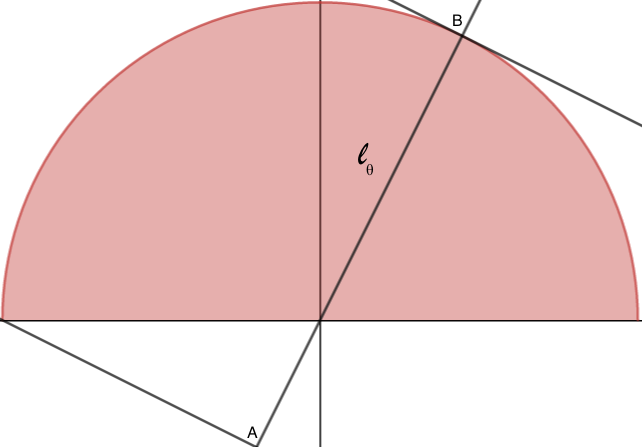
\includegraphics[scale=0.3]{semicircle-1.png}
                \caption{Caption}
                \label{fig:my_label}
            \end{figure}
            \begin{definition}
            A functional $f$ with respect to subset inclusion is said to be monotonic on a family of sets $\mathscr{P}$ if and only if $f(K)\leq f(L)$ for all $K,L \in \mathscr{P}$ such that $K\subset L$.
            \end{definition}
            \begin{theorem}
            If $K\subset L \in \mathscr{K}_2$, then $W_{\ell}(K) \leq W_{\ell}(L)$.
            \end{theorem}
            \begin{proof}
            For let $\pi_{\ell}:\mathbb{R}^2 \rightarrow \ell$ be the orthogonal projection map of $\mathbb{R}^2$ to $\ell$. Then $\pi_{\ell}(K)\leq \pi_{\ell}(L)$ as $K\subset L$, and thus $W_{\ell}(K)\leq W_{\ell}(L)$.
            \end{proof}
            \begin{theorem}
            If $K\subset L\in \mathscr{K}_2$, then $W(K)\leq W(L)$.
            \end{theorem}
            \begin{proof}
            For $W_{\ell}(K)\leq W_{\ell}(L)$, and thus $W(K)=\frac{1}{2\pi}\int_{0}^{2\pi}W_{\ell_{\theta}}(K)d\theta \leq \frac{1}{2\pi}\int_{0}^{2\pi}W_{\ell_{\theta}}(L)d\theta=W(L)$.
            \end{proof}
            \begin{theorem}
            If $K\subset L\in \mathscr{K}_2$, then $X_{\ell}(K)\leq X_{\ell}(L)$.
            \end{theorem}
            \begin{proof}
            For if $x\in \ell\cap K$, then $x\in \ell\cap L$, and thus $X_{\ell}(K)=\mu(\ell\cap K) \leq \mu(\ell\cap L)=X_{\ell}(L)$.
            \end{proof}
            \begin{theorem}
            If $K\subset L\subset \mathscr{K}_2$, then $D(K)\leq D(L)$.
            \end{theorem}
            \begin{proof}
            For suppose not. Suppose $D(K)>D(L)$. Then, there are points $x,y\in K$ such that $d(x,y)> \sup\{d(x',y'):x',y'\in L\}$. But as $K\subset L$, $x,y\in L$ and thus $d(x,y) \not> \sup\{d(x',y'):x',y'\in L\}$. Thus, $D(K)\leq D(L)$.
            \end{proof}
            \begin{theorem}
            If $K\subset L \subset \mathscr{K}_2$, then $R_K\leq R_L$.
            \end{theorem}
            \begin{proof}
            For suppose not. Suppose $R_K>R_L$. But as $K\subset L$, either this circle contains all of $L$ as well or it doesn't. But then $R_L \not<R_K$. Thus, $R_L\geq R_K$.
            \end{proof}
            \begin{theorem}
            If $K\subset L \in \mathscr{K}_2$, then $r_K \leq r_L$.
            \end{theorem}
            \begin{proof}
            For suppose not. Suppose $r_K> r_L$. But as the inscribed circle of radius $r_K$ fits entirely in $K$, and $K\subset L$, then it fits inside of $L$. But then $r_K \not > r_L$. Thus, $r_L \geq r_K$.
            \end{proof}
            \begin{theorem}
            If $K,L\in \mathscr{K}_2$ and $K\subset L$, then $P(K)\leq P(L)$.
            \end{theorem}
            \begin{proof}
            As $K\subset L\in  \mathscr{K}_2$, $W(K)\leq W(L)$. As $K$ and $L$ are convex, $P(K)=\pi W(K)$ and $P(L)=\pi W(L)$. Thus, $P(K) \leq \pi W(L) = P(L)$. Therefore, $P(K)\leq P(L)$.
            \end{proof}
            \begin{theorem}
            There exists sets $K,L\subset \mathbb{R}^2$ such that $L$ is convex, $K\subset L$, yet $P(K)>P(L)$.
            \end{theorem}
            \begin{proof}
            For let $L = \{(x,y)\in \mathbb{R}^2: x^2 + y^2 \leq 1\}$. Then $P(L) = 2\pi$. Let $K = \{(x,y)\in \mathbb{R}^2: -\sqrt{2}x\leq y \leq \sqrt{2}x,\frac{-1}{\sqrt{3}} \leq x \leq \frac{1}{\sqrt{3}} \lor \sqrt{2}x\leq y \leq -\sqrt{2}x,\frac{-1}{\sqrt{3}} \leq x \leq \frac{1}{\sqrt{3}} \}$. $P(K) = 4(1+ \sqrt{\frac{2}{3}}) \approx 7.26>2\pi$.
            \end{proof}
            \begin{figure}[H]
              \begin{subfigure}[b]{0.49\textwidth}
                 \centering
                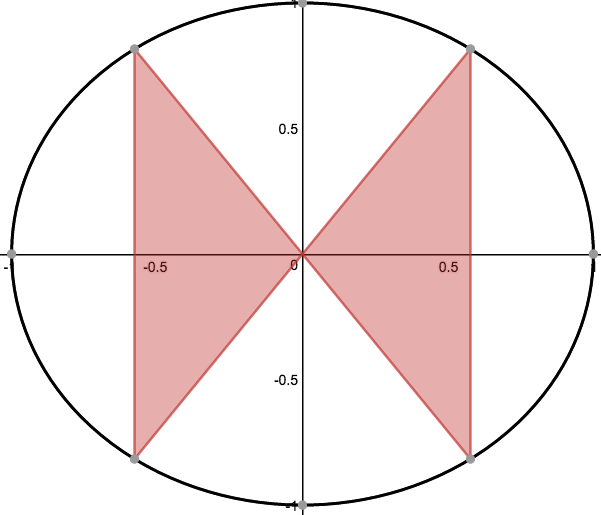
\includegraphics[width=\textwidth]{Circles-3.png}
                \caption{Drawing for Theorem 3.2.15}
              \end{subfigure}
              \begin{subfigure}[b]{0.49\textwidth}
                \centering
                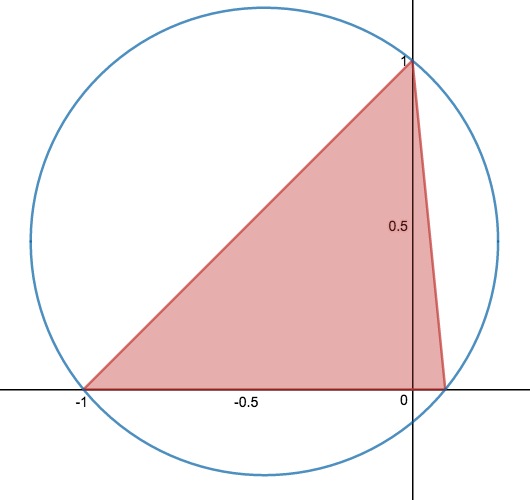
\includegraphics[width=\textwidth]{Circle-4.png}
                \caption{Drawing for Theorem 3.2.16}
              \end{subfigure}
            \end{figure}
            \begin{theorem}
            There exist compact convex sets in $\mathbb{R}^2$ such that $D(K) < 2R_K$.
            \end{theorem}
            \begin{proof}
            For consider the set $K=\{(x,y)\in \mathbb{R}^2: [0\leq y\leq x+1 \land x\geq 0]\lor [0\leq y\leq -10x+1\land x\geq 0]\}$. From Euclid, the smallest circle containing this triangle is the one defined by the three vertices (Three points define a triangle). This circle has the formula $(x+0.45)^2+(y-0.45)^2 = (0.45)^2 +(0.45+\frac{1}{10})^2$. Thus, $2R_K = \sqrt{0.45^2 +(0.45+\frac{1}{10})^2} > \sqrt{2} = D(K)$.
            \end{proof}
            \begin{theorem}
            If $K$ is a compact convex set in $\mathbb{R}^2$, then $D(K) \leq 2R_K$.
            \end{theorem}
            \begin{proof}
            For suppose not. Suppose $D(K) > 2R_K$. As $K$ is compact, there are points $x$ and $y$ in $K$ such that $d(x,y)=D(K)$. But then $d(x,y)>2R_K$, and thus at least one of $x$ or $y$ is not contained in the circle. A contradiction. Thus $D(K)\leq 2R_K$.
            \end{proof}
            \begin{theorem}
            If $K$ is a compact convex set in $\mathbb{R}^2$, then $2\pi r_K \leq P(K)$.
            \end{theorem}
            \begin{proof}
            From Calculus of Variations we know that the circle maximizes the area contained with a set of perimeter $p$. As the inscribed circle has perimeter $2\pi r_K$ and as the circle is a subset of $K$, it is true that $A(K)$ is greater than or equal the area of the circle. Thus, $P(K)\geq 2\pi r_K$.
            \end{proof}
            \begin{theorem}
            For a compact convex set of $\mathbb{R}^2$, $P(K) \leq 2\pi R_K$.
            \end{theorem}
            \begin{proof}
            As $K$ is convex, $P(K) = \pi W(K) \leq \pi \check{W}(K) = \pi D(K) \leq 2\pi R_K$.
            \end{proof}
            \begin{theorem}
            If $K$ is a compact and convex subset of $\mathbb{R}^2$, then $2D(K)\leq P(K)$.
            \end{theorem}
            \begin{proof}
            Suppose not. Suppose $2D(K) >P(K)$. As $K$ is compact and convex, there exist points $x,y\in K$ such that $d(x,y) = D(K)$. But as $K$ is convex, the line contained between $x,y$ in contained in $K$. Thus, $P(\overline{xy}) = 2D(K)$. But as $\overline{xy}\subset K$, $P(K)>P(\overline{xy})$, a contradiction. Thus, $2D(K) \leq P(K)$.
            \end{proof}
            \begin{theorem}
            There exist compact convex subsets of $\mathbb{R}^2$ such that $2D(K) = P(K)$.
            \end{theorem}
            \begin{proof}
            For take a straight line segment of length $\ell$. Then $D(K) = \ell$, $P(K) = 2\ell$, and thus $2D(K) = P(K)$.
            \end{proof}
            \begin{theorem}
            If $K$ is a compact convex subset of $\mathbb{R}^2$, then $P(K) \leq \pi D(K)$.
            \end{theorem}
            \begin{proof}
            From Cauchy's Perimeter theorem, $P(K) = \pi W(K) \leq \pi \check{W}(K) = \pi D(K)$.
            \end{proof}
            \begin{theorem}
            For a compact convex subset $K$ of $\mathbb{R}^2$, $P(K) = \pi D(K)$ if and only if $W_{\ell}(K)$ is a constant.
            \end{theorem}
            \begin{proof}
            For then $\frac{1}{2\pi} \int_{0}^{2\pi} W_{\ell_{\theta}}(K) d\theta = \check{W}(K)$. But as $W_{\ell_{\theta}}(K)$ is continuous for compact convex bodies, it must be true that $W_{\ell_{\theta}}(K) = \check{W}(K)$ for all $\ell_{\theta}$. Thus, $K$ is of constant width.
            \end{proof}
            \begin{remark}
            There are many types of shapes that have constant width besides discs. The Reuleaux Triangle is such an example.
            \end{remark}
            Triangles are the simplest convex bodies in the plane other than points and lines. Any convex polygon can be written as the union of triangles with disjoint interiors. 
            \begin{theorem}
            If $\Delta_s$ is an equilateral triangle with edge length $s$, then $\Delta_s$ has the following properties:
            \begin{enumerate}
            \begin{multicols}{5}
            \item $A(\Delta_s) = \frac{\sqrt{3}}{4}s^2$
            \item $P(\Delta_s) = 3s$
            \item $W(\Delta_s) = \frac{3s}{\pi}$
            \item $R_{\Delta_s} = \frac{1}{\sqrt{3}}s$
            \item $r_{\Delta_s} = \frac{1}{2\sqrt{3}}s$
            \end{multicols}
            \end{enumerate}
            \end{theorem}
            \begin{proof}
            In order:
            \begin{enumerate}
                \item From Pythagoras, $A(\Delta_s) =2\times\big[\frac{1}{2}(\frac{1}{2}s)(\frac{\sqrt{3}}{2}s)\big] = \frac{\sqrt{3}}{4}s^2$
                \item There are three edges, each of length $s$, and thus $P(\Delta_s) = 3s$.
                \item $W(\Delta_s) = \frac{1}{\pi}P(\Delta_s) = \frac{3s}{\pi}$
                \item The circumcircle gives the following equations:
                \begin{enumerate}
                    \item $R_{\Delta_s}^2=\frac{s^2}{4}+h^2$
                    \item $h+R_{\Delta_s} = \frac{\sqrt{3}}{2}s$
                \end{enumerate}
                This has solution $R_{\Delta_s}=\frac{1}{\sqrt{3}}s$
                \item $r_{\Delta_s} = \frac{R_{\Delta_s}}{2}= \frac{1}{2\sqrt{3}}s$
            \end{enumerate}
            \end{proof}
            \begin{theorem}
            If $T$ is a triangle in the plane, then there is a linear transformation $\psi$ such that $\psi T$ is equilateral.
            \end{theorem}
            \begin{proof}
            For let $T$ be a triangle with vertices $a=(x_1,y_1)$, $b=(x_2,y_2)$, $c=(x_3,y_3)$. Let $A = d(b,c)$, $B=d(a,c)$, and $C=d(a,b)$. Suppose If $A=B=C$, we are done. Thus, suppose $C\geq B >A$. At point $a$ and with radius $C$, construct the circle $b,c',d$, and point $b$ and with radius $C$, construct the circle $a,c',e$. If we can shift $c$ to $c'$ in a linear fashion, we are done. Let $\psi =$
            \end{proof}
            \begin{theorem}
            If $T$ is a triangle with edges $a,b,c$ and opposite angles $\alpha,\beta,\gamma$, respectively, then $A(T) = \frac{\sin(\alpha)}{2}bc = \frac{\sin(\beta)}{2}ac = \frac{\sin(\gamma)}{2}ab$
            \end{theorem}
            \begin{proof}
            Suppose the triangle is acute. The proof is symmetric for all sides, so we prove it for just $\alpha$. Note that the perpendicular $h$ dropped from the vertex of $a$ onto $b$ satisfies $h^2+\ell_1^2 = c^2$ and $h^2+\ell_2^2 = a^2$, where $\ell_1+\ell_2 = b$. Then $\sin(\alpha) = \frac{h}{c}$ and $A(T) = \frac{1}{2}h\ell_1 + \frac{h}{2}h\ell_2 = \frac{h}{2}(\ell_1+\ell_2)h = \frac{1}{2}bh = \frac{1}{2}bc\sin(\alpha)$. An identical argument works for obtuse triangles.
            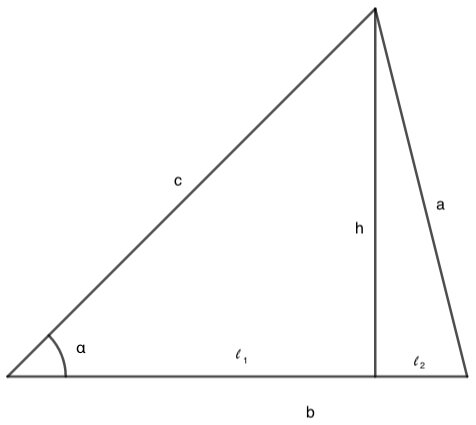
\includegraphics[scale=0.3]{triangle-1.png}
            \end{proof}
            \begin{corollary}[The Law of Sines]
            For a triangle with edges $a,b,c$ and opposite angles $\alpha,\beta,\gamma$, $\frac{\sin(\alpha)}{a} = \frac{\sin(\beta)}{b} = \frac{\sin(\gamma)}{c}$
            \end{corollary}
            \begin{proof}
            From the previous theorem, divide by $\frac{abc}{2}$ to obtain the result.
            \end{proof}
            \begin{theorem}[The Law of Cosines]
            Given a triangle with lengths $a,b,c$ and opposite edges $\alpha,\beta,\gamma$, $c^2=a^2+b^2-2ab\cos(\gamma)$.
            \end{theorem}
            \begin{proof}
            If $\gamma=\frac{\pi}{2}$, this is Pythagoras' Theorem. Thus, suppose $0<\gamma < \frac{\pi}{2}$. Where $c$ and $a$ meet, drop a perpendicular onto $c$ and call this $h$. $h$ satisfies $h^2+\ell_1^2 = c^2$ and $h^2+\ell_2^2=a^2$ from Pythagoras' Theorem, where $\ell_1+\ell_2 = b$. But $\ell_2 = a\cos(\gamma)$, so $\ell_1 = b-a\cos(\gamma)$. Thus $c^2 = h^2 + b^2 +a^2\cos^2(\gamma)-2ab\cos(\gamma)$. But $h = a\sin(\gamma)$. Thus, $c^2 = b^2 + a^2 \cos^2(\gamma)+\sin^2(\gamma)-2ab\cos(\gamma) = b^2 + a^2(\sin^2(\gamma)+\cos^2(\gamma))-2ab\cos(\gamma) = a^2 + b^2 -2ab\cos(\gamma)$. A similar construction is done if $\frac{\pi}{2}<\gamma < \pi$.
            \end{proof}
            \begin{theorem}
            Given a triangle $\Delta$ with lengths $a\leq b\leq c$, $D(\Delta)=c$.
            \end{theorem}
            \begin{proof}
            At the midpoint of $c$, and with radius $c$, construct a circle. This circle contains the entirety of $\Delta$, and thus for all points $x,y\in \Delta$, $d(x,y)\leq c$. Thus, $c=D(\Delta)$.
            \end{proof}
            \begin{theorem}[Heron's Formula]
            For a triangle with lengths $a,b,c>0$, $A(T)^2 = \frac{1}{16}(a+b+c)(-a+b+c)(a-b+c)(a+b-c)$.
            \end{theorem}
            \begin{proof}
            For $A(T) = \frac{1}{2}ab \sin(\gamma) = \frac{1}{2}ab\sqrt{1-\cos^2(\gamma)} = \frac{1}{4}\sqrt{4a^2 b^2 - (a+b-c)^2}=\\ \frac{1}{4}\sqrt{(2ab-(a^2+b^2-c^2))(2ab+(a^2+b^2+c^2))} = \frac{1}{4}\sqrt{(c^2-(a-b)^2)((a+b)^2-c^2)} = \\ \frac{1}{4}\sqrt{(a+b+c)(-a+b+c)(a-b+c)(a+b-c)}$. Squaring this gives the result.
            \end{proof}
            \begin{theorem}
            For any triangle $\Delta$, $r_{\Delta}P(\Delta) = 2A(\Delta)$.
            \end{theorem}
            \begin{proof}
            For let $\Delta$ has sides $a,b,c$, with opposite angles $\alpha, \beta, \gamma$, respectively. Then $A(\Delta) = \frac{ab}{2}\sin(\gamma)$ and $P(\Delta)=a+b+c$. Thus, $\frac{2A(\Delta)}{P(\Delta)} = \frac{ab\sin(\gamma)}{a+b+c}$. But this is the radius of the incircle of $\Delta$. Therefore, etc.
            \end{proof}
            \begin{theorem}[Viviani's Theorem: Page 17]
            \end{theorem}
            \begin{theorem}
            There exist convex polygon's such that the inradius is not unique.
            \end{theorem}
            \begin{proof}
            For consider the rectangle $[0,2]\times [0,1]$. The diameter of any circle that sits inside this body must be at most $1$, and thus the radius is at most $\frac{1}{2}$. However, there are multiple circles that achieve this. For example $(x-\frac{1}{2})^2+(y-\frac{1}{2})^2=\frac{1}{2}$ and $(x-\frac{3}{2})^2+(y-\frac{3}{2})^2=\frac{1}{2}$.
            \end{proof}
            \begin{theorem}
            For an acute triangle, $\frac{2(A)}{abc} = \frac{1}{R_T}$.
            \end{theorem}
            \begin{theorem}
            If $\Delta$ is a triangle with vertices $A,B,C$ and sides $a,b,c$, then given a circle that contains $A,B,C$, the radius of this circle $R$ satisfies $\frac{1}{R} =\frac{2A(\Delta)}{abc}$
            \end{theorem}
            \begin{definition}
            If $K\in \mathscr{K}_2$, then $-K = \{-x:x\in K\}$.
            \end{definition}
            \begin{theorem}
            If $K\in \mathscr{K}_2$, then $W_{\ell}(K) = W_{\ell}(-K)$.
            \end{theorem}
            \begin{proof}
            For let $x,y\in K$ be such that $d(x,y) = W_{\ell}(K)$. Then $d(-x,-y) = W_{\ell}(-K) = d(x,y)$. Therefore, etc.
            \end{proof}
            \begin{theorem}
            There exist sets $K$ and $L$ such that $W_{\ell}(K)<W_{\ell}(L)$ for all $\ell$ yet $K\not\subset L$ for any translation or rotation of $K$.
            \end{theorem}
            \begin{definition}
            For $K\in \mathscr{K}$ and unit vector $u$, $\bar{X}_{u}(K)$ is the mean value of $X_{\ell}(K)$ over all lines $\ell$ parallel to $u$ such that $X_{\ell}(K)>0$.
            \end{definition}
            \begin{theorem}
            For $K\in \mathscr{K}_2$, $\bar{X}_{u}(K) = W_{\ell}(K)=A(K)$.
            \end{theorem}
        \section{On Uniform Convergence}
            \begin{definition}
                A sequence of functions $f_n$ is said to converge
                point-wise on a set $A$ to a function $f$, if
                $\forall\varepsilon>0$ and $\forall x\in A$, there is
                an $N\in\mathbb{N}$ such that $n>N \Rightarrow
                |f(x)-f_n(x)|<\varepsilon$.
            \end{definition}
            \begin{definition}
                A sequence of functions $f_n$ converge uniformly on a
                set $A$ to $f$ if and only if $\forall \varepsilon>0$
                $\exists N\in\mathbb{N}$ such that $\forall x \in A$
                and $n>N$, $|f(x) -f_n(x)|<\varepsilon$.
            \end{definition}
            \begin{definition}
                A sequence of functions $f_n$ are point-wise
                equicontinuous on a set $A$ if and only if
                $\forall_{\varepsilon>0}\forall_{x\in A}
                \exists_{\delta>0}\forall_{n\in\mathbb{N}}:
                |x-x_0|<\delta\Rightarrow|f_{n}(x)-f_{n}(x_0)|<
                \varepsilon$
            \end{definition}
            \begin{definition}
                A sequence of functions $f_n$ are uniformly
                equicontinuous on a set A if and only if
                $\forall_{\varepsilon>0}\exists_{\delta>0}
                \forall_{x\in A}\forall_{n\in\mathbb{N}}:
                |x-x_{0}|<\delta\Rightarrow|f_{n}(x)-f_{n}(x_{0})|<
                \varepsilon$.
            \end{definition}
            \begin{definition}
                A subset $A$ of the real line is open if
                $\forall_{x\in A}\exists_{r>0}:
                \forall_{y\in (x-r,x+r)},y\in A$.
            \end{definition}
            \begin{definition}
                An open cover $\Delta$ of a set $A\subset S$ is a set
                of open subsets $A_k\subset S$, such that
                $A\subset\cup_{k\in I}A_{k}$, where $I$ is some
                index, countable or uncountable.
            \end{definition}
            \begin{definition}
                A set $A$ is said to be compact if and
                only if for all open coverings $\Delta$ there is
                a finite sub-cover $\Delta_0\subset \Delta$, such
                that $A\subset \cup_{A_k \in \Delta_0} A_k$.
            \end{definition}
            \begin{theorem}
                [Heine-Borel Theorem]
                Any closed-bounded subset of the real line is compact. 
            \end{theorem}
            \begin{proof}
                For let $A$ be a closed and bounded subset of
                $\mathbb{R}$ with least upper bound $b$ and
                greatest lower bound $a$. Let $\Delta$ be an
                open covering, and let $X$ be the set of
                points $y\in A$ such that for all $s<y$ such
                that $s\in A$, there is a finite refinement
                of $\Delta$ which covers these points. $X$ is
                non-empty, as $a\in X$. The set $X$ is bounded,
                as for all points $y\in X$ we have that
                $a\leq y\leq b$. As bounded sets have a least
                upper bound, let $x$ be the least upper bound.
                Suppose $x<b$. As $x\in [a,b]$, there exists an
                element $A_k$ of $\Delta$ such that $x \in A_k$.
                But as $A_k$ is open and therefore there is an
                $r>0$ such that
                $y\in (x-r,x+r)\Rightarrow y \in A_k$.
                But then $y=x+\frac{r}{2}>x$ and
                $y\in A_k$. Therefore x is not the
                least upper bound as we have found an
                element in $X$ greater than $x$.
                Therefore $x\not<b$. And thus $x=b$.
            \end{proof}
            \begin{theorem}
                If a sequence of functions are
                point-wise equicontinuous on a closed
                and bounded set, then they are
                uniformly equicontinuous.
            \end{theorem}
            \begin{proof}
                For let $A$ be a closed bounded subset
                of $\mathbb{R}$, and let $f_n(x)$ be a sequence
                of point-wise equicontinuous functions on $A$.
                As the set is closed and bounded, it is compact
                by the Heine-Borel theorem. Let $\varepsilon>0$
                be given. For $x\in A$, define the function
                $\delta(x)%
                 =\min\{\sup\{\delta>0:|x-x_0|<\delta,\ x_0\in A%
                  \Rightarrow |f_n(x)-f_n(x_0)|<\frac{\varepsilon}{2}$,
                $\forall n\in\mathbb{N}\},b-a\}$.
                Construct the open covering $\mathcal{U}$ as
                follows:
                $\mathcal{U}=\{(x-\delta(x),x+\delta(x)):\ x\in A\}$.
                This is an open covering, as every set in
                $\mathcal{U}$ is open, and for all
                $x\in A$, $x\in(x-\delta(x),x+\delta(x))\in\mathcal{U}$.
                But as $A$ is compact, there is a finite sub-cover.
                Let $a=x_0<x_1<...<x_{n-1}<x_n=b$ be the centers
                of the remaining open sets in the sub-cover.
                Further refine this sub-covering as follows: If
                $(x_j-\delta(x_j),x_j+\delta(x_j))%
                 \subset (x_k-\delta(x_k),x_k+\delta(x_k))$
                for $j\ne k$, then remove it from the sub-cover as
                it is superfluous. We now have a set of points
                $a=z_0<z_1<...<z_{N-1}<z_N=b$ such that
                $A\subset\cup_{i=0}^{N} (z_i-\delta(z_i),z_i+\delta(z_i))$.
                Let
                $\delta%
                 =\min\{\delta(z_0),...,\delta(z_N),\delta(b),%
                        \frac{(a+\delta(a))-(z_1-\delta(z_1))}{2},%
                        ...,%
                        \frac{(z_{N-1}+\delta(z_{N-1}))-(b-\delta(b))}{2}\}$.
                That is, $\delta$ is the smallest of the $\delta(z_i)$,
                or half of the smallest intersection of two consecutive
                intervals. Let $x\in A$ be arbitrary. If $(x-\delta,x+\delta)$
                is contained entirely in one of the
                $(z_i-\delta(z_i),z_i+\delta(z_i))$ sets, then we have
                that $|x-x_0|<\delta \Rightarrow |x-x_0| <\delta(z_i) \Rightarrow |f_n(x)-f_n(x_0)|<\frac{\varepsilon}{2}$ for all $n\in\mathbb{N}$.
                Suppose that $(x-\delta,x+\delta)$ is contained in two of
                the $(x-\delta(z_i),x+\delta(z_i))$ sets. Note, it cannot
                be in three or more as we have refined the sub-cover in
                such a manner as to prevent this. Let $y$ be the center
                of the intersection of these two sets. Then we have that
                for $|x-x_0|<\delta$, then
                $|f_n(x)-f_n(x_0)|%
                 =|f_n(x)-f_n(y)+f_n(y)-f_n(x_0)|%
                 \leq|f_n(x)-f_n(y)|+|f_n(y)-f_n(x_0)|$.
                But $|x-y|$ and $|x_0-y|$ are less than
                $\frac{(z_i + \delta(z_i))-(z_{i+1}-\delta(z_{i+1}))}{2}$
                apart, and therefore $|f_n(x)-f_n(y)|<\frac{\varepsilon}{2}$,
                and $|f_n(y)-f_n(x_0)|<\frac{\varepsilon}{2}$.
                Therefore, $|f_n(x)-f_n(x_0)|<\varepsilon$.
                And as $x$ is arbitrary,
                $f_n(x)$ is uniformly equicontinuous.
            \end{proof}
            \begin{theorem}
                If a sequence of point-wise equicontinuous functions converge, then the limit is point-wise continuous.
            \end{theorem}
            \begin{proof}
                For let $f_n:A\rightarrow \mathbb{R}$ be equicontinuous, $\varepsilon>0$ and $x\in A$ be given. Choose $\delta>0$ to satisfy the criterion of equicontinuity at $x$. Let $x_0$ be an arbitrary point in $(x-\delta,x+\delta)\cap A$. It suffices to show that $|f(x) - f(x_0)|<\varepsilon$. As $f_n \rightarrow f$ we have that $\exists N_1 \in\mathbb{N}$ such that $n>N_1\Rightarrow |f(x) - f_n(x)|<\varepsilon$. We also have that $\exists N_2 \in \mathbb{N}$ such that $n>N_2 \Rightarrow |f(x_0)-f_n(x_0)|<\varepsilon$. Let $N=\max\{N_1,N_2\}+1$. But we have that $|f(x) - f(x_0)| = |f(x) - f_N(x) + f_N(x)-f_N(x_0) + f_N(x_0) - f(x_0)|\leq |f(x) - f_n(x)| + |f_n(x)-f_n(x_0)| + |f_n(x_0) - f(x_0)| < 3\varepsilon$. $f$ is continuous.
            \end{proof}
            \begin{theorem}
                If $f_n \rightarrow f$ on a closed bounded subset of $\mathbb{R}$, and if $f_n$ is equicontinuous, then the convergence is uniform.
            \end{theorem}
            \begin{proof}
                Let $A$ be a closed bounded subset of $\mathbb{R}$, $f_n(x)$ a sequence of equicontinuous functions, and let $\varepsilon>0$ be given. As $f_n(x)$ is equicontinuous on a closed bounded set, it is uniformly equicontinuous. But the limit of equicontinuous functions is continuous. Let $\delta>0$ be such that, $\forall x\in A$, $\forall n\in\mathbb{N}$, $|x-x_0|<\delta, x_0\in A \Rightarrow |f_n(x)-f_n(x_0)|<\frac{\varepsilon}{3}$ and $|x-x_0|<\delta \Rightarrow |f(x)-f(x_0)|<\frac{\varepsilon}{3}$. Let $\mathcal{U} = \{(x-\frac{\delta}{2},x+\frac{\delta}{2}): x\in A\}$. This is an open cover of $A$ and thus there is a finite subcover. Let $x_0<x_1<\hdots<x_n$ be the centers of the finitely many sets $(x_k-\frac{\delta}{2},x_k+\frac{\delta}{2})$ that cover $A$. There is thus another finite sequence of positive integers, $N_0, N_1,... N_n$, such that $n>N_k \Rightarrow |f(x_k)-f_n(x_k)|<\frac{\varepsilon}{3}$, for $k=0,1,2,...,n$. Let $N= \max\{N_0, N_1, ..., N_n\}$.It suffices to show that, for any point $x_0 \in A$, for all $n>N$, $|f(x_0)-f_n(x_0)|<\varepsilon$. Let $x_0$ be arbitrary and let $x_k$ be the nearest point to $x_0$ in the above sequence (If there are two nearest points, pick your favorite). Then we have that, for $n>N$, $|f(x_0) - f_n(x_0)| = |f(x_0)-f(x_k)+f(x_k)-f_n(x_k)+f_n(x_k)-f_n(x_0)|\leq |f(x_k)-f(x_0)|+|f(x_k)-f_n(x_k)|+|f_n(x_k)-f_n(x_0)|<\varepsilon$. The convergence is uniform.
            \end{proof}
            \begin{theorem}
                [Integration of a Uniformly Convergent Sequence of Functions]
                If $f_n\rightarrow f$ uniformly on a closed bounded set $A$ with $g.u.b(A)=a$, then $\int_{a}^{x} f_n \rightarrow \int_{a}^{x} f$ uniformly on $A$.
            \end{theorem}
            \begin{proof}
                Let $\varepsilon >0$ be given, let $b=l.u.b.(A)$, and choose $N\in\mathbb{N}$ such that $n>N\Rightarrow |f(x)-f_n(x)|<\frac{\varepsilon}{b-a}$. Then we have $|\int_{a}^{x} f_n - \int_{a}^{x} f| = |\int_{a}^{x} (f_n-f)| \leq \int_{a}^{x} |f_n-f| < \int_{a}^{x} \frac{\varepsilon}{b-a}= \frac{\varepsilon}{b-a}(x-a) \leq \varepsilon$.
            \end{proof}
            \begin{theorem}
                [Differentiation of a Uniformly Convergent Sequence of Functions]
                If $f_n'\rightarrow g$ uniformly on a closed bounded set $A$, and if $f_n \rightarrow f$ on $A$, then $f'=g$.
            \end{theorem}
            \begin{proof}
                Let $a=g.u.b.(A)$ and $b=l.u.b.(A)$. We have that $f_n(x) - f_n(a) = \int_{a}^{x}f_n' \rightarrow \int_{a}^{x}g$ uniformly. But $f_n(x)-f_n(a) \rightarrow f(x) - f(a)$. Therefore $f'(x)=\frac{d}{dx}(f(x)-f(a)) = \frac{d}{dx}\int_{a}^{x} g = g(x)$. $f' = g$.
            \end{proof}
            \begin{theorem}
                [The Product of a Uniformly Convergence Sequence and a Bounded Function]
                If $f_n \rightarrow f$ uniformly, and if $g$ is a bounded function, then $f_n g \rightarrow fg$ uniformly.
            \end{theorem}
            \begin{proof}
                For let $\varepsilon>0$ and $x$ be given, and let $g$ be a bounded function with bound $M$, and choose $N\in\mathbb{N}$ such that $n>N \Rightarrow |f(x)-f_n(x)|<\frac{\varepsilon}{M}$. Then we have that $|f(x)g(x)-f_n(x)g(x)| = |g(x)||f(x)-f_n(x)| < M|f(x)-f_n(x)| <\varepsilon$.
            \end{proof}
            \begin{theorem}
                If $f$ is continuous on a compact set $A$, then it is uniformly continuous.
            \end{theorem}
            \begin{proof}
                For let $\varepsilon>0$ be given, let $a=g.u.b.(A)$, $b=l.u.b.(A)$, and for $x\in A$ define $\delta(x) = \min\{\sup\{\delta>0: |x-x_0|<\delta,x_0\in A\Rightarrow |f(x)-f(x_0)|<\frac{\varepsilon}{2}\},b-a\}$. Let $\Delta = \{(x-\delta(x),x+\delta(x)):x\in A\}$. Then $\Delta$ is an open cover of $A$ and therefore there is an open subscover. Let $x_k$ be the centers of the finitely many sets $(x_k-\delta(x_k),x+\delta(x_k))$ that cover $A$. Further refine this by removing overlaps. That is, if $(x_i-\delta(x_i),x_i+\delta(x_i))\subset (x_j-\delta(x_j),x_j+\delta(x_k))$ for $i\ne j$, then remove it for it is superfluous. We thus obtain a new sequence $z_1,\hdots, z_N$ such that the intervals $(z_k-\delta(z_k),z_k+\delta(z_k))$ cover $A$. Define $\delta = \min\{\delta(z_1),\hdots,\delta(z_N), \frac{(z_0+\delta(z_0))-(z_1-\delta(z_1))}{2},\hdots,(\frac{z_{N-1}+\delta(z_{N-1}))-(z_{N}-\delta(z_{N})}{2}\}$. Let $x,x_0\in A$ such that $|x-x_0|<\delta$. Let $x_k$ be the closest point in the sequence to $x$ (If there are two such points, pick your favorite). Then $|f(x)-f(x_0)|=|f(x)-f(x_k)+f(x_k)-f(x_0)|\leq |f(x)-f(x_k)|+|f(x_k)-f(x_0)|<\varepsilon$
            \end{proof}
            \begin{remark}
                The proof of this is a mimicry of the proof that equicontinuity on a compact set implies uniform equicontinuity.
            \end{remark}
            \begin{definition}
                A set $A$ is called sequentially compact if given a sequence $x_n\in A$, there is a convergent subsequence $x_{n_k}$.
            \end{definition}
            \begin{theorem}
                Compact sets of $\mathbb{R}$ are sequentially compact.
            \end{theorem}
            \begin{proof}
                Let $A$ be a compact set in $\mathbb{R}$, and let $x_n$ be a sequence in $A$. A point $x\in A$ is the limit of a subsequence of $x_n$ if for every $\varepsilon>0$ there are infinitely many of the $x_n$ such that $|x-x_n|<\varepsilon$. Suppose there is no such point. That is, for each $x\in A$ only finitely many of the $x_n$ lie within sufficiently small $\varepsilon-$neighborhoods. Let $\varepsilon(x) = \sup\{\varepsilon>0:\textrm{Only finitely many }x_n \textrm{ lie within } \varepsilon \textrm{ of } x\}$. Define $E=\{(x-\varepsilon(x)<x+\varepsilon(x)):x\in A\}$. This is an open cover of $A$, and therefore there is a finite subcover. Thus, at least one of the finitely many intervals $(x-\varepsilon(x),x+\varepsilon(x))$ must contain infinitely many of the $x_n$, a contradiction. Thus there is a convergent subsequence.
            \end{proof}
            \begin{theorem}
                Continuous functions on compact sets are bounded.
            \end{theorem}
            \begin{proof}
                For suppose not. Let $f:A\rightarrow \mathbb{R}$ be a continuous function on a compact set $A$, and let $x_n$ be a sequence of points in $A$ such that $f(x_n)>n$. Such a sequence must exist as $f$ is not bounded. As $A$ is compact, there must a point $x\in A$ such that some subsequence $x_{n_k}$ that converges to $x$. Let $\varepsilon >0$. Then, as $f$ is continuous, there is a $\delta>0$ such that $|x-x_0|<\delta,\ x_0\in A\Rightarrow |f(x)-f(x_0)|<\varepsilon$. But then for all points $x_{n_k}$ such that $|x-x_{n_k}|<\delta$, $-\varepsilon<f(x_{n_k})-f(x)<\varepsilon \Rightarrow f(x)-\varepsilon < f(x_{n_k})<f(x)+\varepsilon$. A contradiction as $f(x_{n_k})$ is unbounded. Thus, $f$ is bounded.
            \end{proof}
            \begin{corollary}
                Continuous functions on compact sets attain their maximum and minimum.
            \end{corollary}
            \begin{proof}
                For let $f:A\rightarrow \mathbb{R}$ be a continuous function on a compact set $A$. Let $f(A) = \{y\in \mathbb{R}:\exists x\in A|\ f(x)=y\}$. (This is called the image of $A$ under $f$). As $f$ is continuous, it is bounded, and thus the set $f(A)$ is bounded. But bounded sets have an l.u.b. and a g.u.b. Therefore, etc.
            \end{proof}
            \begin{lemma}
                [Uniform Limit Theorem]
                If $f_n\rightarrow f$ uniformly, and if the $f_n$ are continuous, then $f$ is continuous.
            \end{lemma}
            \begin{proof}
                For let $\varepsilon>0$ be given and let $x\in A$. Let $N\in \mathbb{N}$ such that $n>N$ implies $|f(\chi)-f_n(\chi)|<\frac{\varepsilon}{3}$ for all $\chi\in A$. Let $\delta>0$ be chosen such that $|x-x_0|<\delta, x_0\in A\Rightarrow |f_N(x)-f_N(x_0)|<\frac{\varepsilon}{3}$. Then  $|f(x)-f(x_0)|=|f(x)-f_N(x)+f_N(x)-f_N(x_0)+f_N(x_0)-f(x_0)|\leq |f(x)-f_N(x_0)|+|f_N(x)-f_N(x_0)|+|f(x_0)-f_N(x_0)|<\varepsilon$.
            \end{proof}
            \begin{theorem}
                If $f_ng\rightarrow fg$ uniformly on a compact set $A$, and if $g$ is continuous and positive, then $f_n\rightarrow f$ uniformly.
            \end{theorem}
            \begin{proof}
                As $g$ is positive on a compact set, its minimum is also positive and is attained on $A$. Let $x_{min}\in A$ be such a minimum of $g$. Let $\varepsilon>0$ be given and let $N\in \mathbb{N}$ be such that for $n>N$, $|f_ng-fg|<\varepsilon\cdot g(x_{min})$. Then, $|f_ng-fg|=|g||f_n-f|\leq |g(x_{min})||f_n-f|<\varepsilon \cdot g(x_{min})\Rightarrow |f_n-f|<\varepsilon$.
            \end{proof}
            \begin{lemma}
                If $f_n'$ is uniformly bounded, then $f_n$ is equicontinuous.
            \end{lemma}
            \begin{proof}
                For let $M$ be such a bound for $f_n'$ and let $\varepsilon>0$ be given. Choose $\delta = \frac{\varepsilon}{M}$. Then for $x,x_0\in A$ and $|x-x_0|<\delta$, $|\int_{x_0}^{x}f_n'| =|f_n(x)-f_n(x_0)| \leq \int_{x_0}^{x}|f_n'| \leq (x-x_0)M < \varepsilon$.
            \end{proof}
            \begin{theorem}
                If $f_n'$ is uniformly bounded, and if $f_n \rightarrow f$ on a closed and bounded subset of $\mathbb{R}$, then the convergence is uniform.
            \end{theorem}
            \begin{proof}
                From the previous lemma, $f_n$ is equicontinuous. But a sequence of equicontinuous functions on a compact set is uniformly equicontinuous. And a sequence of uniformly equicontinuous functions that converge does so uniformly. Therefore, etc.
            \end{proof}
            \begin{theorem}
                If $f_n \rightarrow f$, $f_n'\rightarrow g$ and if $f_n''-f_n'$ is uniformly bounded on a closed bounded set, then the convergences are uniform and $f' = g$.
            \end{theorem}
            \begin{proof}
                Let $A$ be the closed bounded set under consideration. First note that as $f''_n - f'_n$ is uniformly bounded, $f_n'-f_n$ is equicontinuous. But as $f_n'$ and $f_n$ converge to $g$ and $f$, respectively, then $f_n'-f_n$ converges to $g-f$ uniformly. Let $M$ be a bounded for $f_n''-f_n'$. Let $a$ be the greatest lower bound and $b$ be the least upper bound of $A$. We then have that $-Me^{-a}\leq e^{-x}[f_n''(x)-f_n'(x)]=\frac{d}{dx}[e^{-x}f_n'(x)] < Me^{-a}$. That is, $\frac{d}{dx}[e^{-x}f_n'(x)]$ is uniformly bounded, and therefore $e^{-x}f_n'(x)$ is equicontinuous. But equicontinuity on a compact set implies uniform equicontinuity. As $f_n'\rightarrow g$, and $e^{-x}$ is bounded on $A$, $e^{-x}f_n'\rightarrow e^{-x}g$. But a convergent uniformly equicontinuous sequence of functions converges uniformly. Thus, $e^{-x}f_n'(x) \rightarrow e^{-x}g(x)$ uniformly, and therefore, as $e^{-x}$ is continuous and positive on $A$, $f_n'(x)\rightarrow g(x)$ uniformly. But also $f_n'-f_n \rightarrow g-f$ uniformly, and therefore $f_n \rightarrow f$ uniformly. Thus, $f'=g$.
            \end{proof}
            \begin{corollary}
                If $f_n' - f_n$ is uniformly bounded and if $f_n \rightarrow f$ on a closed and bounded set $A$, then the convergence is uniform.
            \end{corollary}
            \begin{proof}
                Using the inequality from the previous theorem, let $M$ be a bound for $f_n'-f_n$ and let $a$ be the least upper bound of $A$. Then $-Me^{-a}\leq \frac{d}{dx}[e^{-x}f_n] \leq Me^{-a}$. Thus $e^{-x}f_n$ is uniformly equicontinuous and therefore $e^{-x}f_n\rightarrow e^{-x}f$ uniformly, and thus $f_n\rightarrow f$ uniformly.
            \end{proof}
            \begin{corollary}
                If $f_n^{(N+1)}-f_n^{(N)}$ is bounded and a compact set, and if $f_n^{(k)}\rightarrow f_k$ for $k=0,1,\hdots, N$, then the convergence is uniform and $f_{k}' = f_{k+1}$ for $k=0,1,\hdots,N-1$.
            \end{corollary}
            \begin{proof}
                A simple induction and application of the previous theorem proves this.
            \end{proof}
        \section{On Analyticity}
            We deal with functions on intervals for simplicity.
            \begin{definition}
                A real-valued function $f$ is said to be smooth, denoted $f\in C^{\infty}$ if, for all $k$, $\frac{d^k}{dx^k}f(x) \equiv f^{(k)}(x)$ exists.
            \end{definition}
        \begin{theorem}[Taylor's Theorem]
        If $f\in C^{\infty}$, on some interval $[a,b]$, and if $x_0\in (a,b)$, then $f(x) - \sum_{k=0}^{n} f^{(k)}(x_0)\frac{(x-x_0)^k}{k!} = \int_{x_0}^{x} f^{(n+1)}(t)\frac{(x-t)^n}{n!}dt$
        \end{theorem}
        \begin{proof}
        We prove by induction. The base case says $f(x)-f(x_0) = \int_{x_0}^{x} f'(t)dt$, which is true. Suppose it holds for some $n\in \mathbb{N}$. Then $f(x)-\sum_{k=0}^{n+1} f^{(k)}(x_0)\frac{(x-x_0)^k}{k!} = f(x)-\sum_{k=0}^{n} f^{(k)}(x_0)\frac{(x-x_0)^k}{k!} - f^{(n+1)}(x)\frac{(x-x_0)^{n+1}}{(n+1)!} = \int_{x_0}^{x} f^{(n+1)}(t)\frac{(x-t)^n}{n!}dt - f^{(n+1)}(x)\frac{(x-x_0)^{n+1}}{(n+1)!}$. But $\int_{x_0}^{x} f^{(n+1)}(t)\frac{(x-t)^n}{n!}dt =  \int_{x_0}^{x} f^{(n+2)}(t) \frac{(x-t)^{n+1}}{(n+1)!} dt + f^{(n+1)}(x)\frac{(x-x_0)^{n+1}}{(n+1)!}$, from integration by parts. Thus, $f(x)-\sum_{k=0}^{n+1} f^{(k)}(x_0)\frac{(x-x_0)^k}{k!}= \int_{x_0}^{x} f^{(n+2)}(t) \frac{(x-t)^{n+1}}{(n+1)!} dt$
        \end{proof}
        \begin{lemma}
        If $f\in C^{\infty}$ and $f^{(n)}(x)\rightarrow 0$ (Point-wise) on $[a,b]$, and if $F(x) \equiv f(x)-\sum_{k=0}^{\infty} f^{(k)}(x_0)\frac{(x-x_0)^{k}}{k!}$, where $x_0\in [a,b]$ is fixed, then $\int_{x_0}^{x} F^{(n+1)}(t)\frac{(x-t)^{n}}{n!}dt$ converges. 
        \end{lemma}
        \begin{proof}
        For let $x,x_0\in [a,b]$ fixed. We will show that $\int_{x_0}^{x} F^{(n+1)}(t)\frac{(x-t)^{n}}{n!}dt$ is Cauchy. Let $\varepsilon>0$, $N_0 = 1$, and let $n>m>N_0$ be arbitrary. We have that $F(x) = \bigg(f(x)-\sum_{k=0}^{N} f^{(k)}(x_0)\frac{(x-x_0)^{k}}{k!}\bigg)-\bigg(g(x)-\sum_{k=0}^{N} f^{(k)}(x_0)\frac{(x-x_0)^{k}}{k!}\bigg)$, where $N\in \mathbb{N}$ is arbitrary. From Taylor's Theorem we thus have $F(x) = \int_{x_0}^{x}F^{N+1}(t)\frac{(x-t)^N}{N!}dt$. Then $|\int_{x_0}^{x}F^{n+1}(t)\frac{(x-t)^n}{n!}dt-\int_{x_0}^{x}F^{m+1}(t)\frac{(x-t)^m}{m!}dt| = |F(x)-F(x)|= 0 <\varepsilon$. 
        \end{proof}
        \begin{theorem}
        If $f\in C^{\infty}$ and $f^{(n)}(x)\rightarrow 0$ (Point-wise) on some interval $[a,b]$, then $f^{(n)}(x)$ is uniformly bounded.
        \end{theorem}
        \begin{proof}
        For let $x_0\in (a,b)$ be arbitrary. As $f^{(n)}(x_0)\rightarrow 0$, $\sum_{k=0}^{\infty} f^{(k)}(x_0)\frac{(x-x_0)^{k}}{k!}$ converges everywhere. Let $g(x)\equiv \sum_{k=0}^{\infty} f^{(k)}(x_0)\frac{(x-x_0)^{k}}{k!}$. Define $F(x) = f(x)-g(x)$. Then:
        \begin{align*}
            F^{(n)}(x) &= f^{(n)}(x)-g^{(n)}(x)\\
            &= \bigg(f^{(n)}(x)-\sum_{k=n}^{N} f^{(k)}(x_0)\frac{(x-x_0)^{k}}{k!}\bigg)-\bigg(g^{(n)}(x)-\sum_{k=n}^{N} f^{(k)}(x_0)\frac{(x-x_0)^{k}}{k!}\bigg)    
        \end{align*}
        From Taylor's theorem, this is equal to:
        \begin{align*}
            \int_{x_0}^{x} f^{(N+n+1)}(t)\frac{(x-t)^{N+n}}{(N+n)!}dt &- \int_{x_0}^{x} g^{(N+n+1)}(t)\frac{(x-t)^{N+n}}{(N+n)!}dt\\
            &= \int_{x_0}^{x} F^{(N+n+1)}(t)\frac{(x-t)^{N+n}}{(N+n)!}dt    
        \end{align*}
        That is, for all $N>n$, $F^{(n)}(x) = \int_{x_0}^{x} F^{(N+n+1)}(t)\frac{(x-t)^{N+n}}{(N+n)!}dt$. But for all $x_1 \in (a,b)$:
        \begin{equation*}
            F^{(n)}(x)-\sum_{k=n}^{N} F^{(k)}(x_1)\frac{(x-x_1)^k}{k!} = \int_{x_1}^{x} F^{(N+n+1)}(t)\frac{(x-t)^{N+n}}{(N+n)!}dt    
        \end{equation*}
        Now, suppose $f^{(n)}(x)$ is not uniformly bounded. $g^{(n)}(x)$ is uniformly bounded by its definition, and thus $F^{(n)}(x)$ is not uniformly bounded. Let ${k_n}$ be a subsequence of $n$ such that $F^{(k_n)}(x_{k_n})>n$. Such a sequence exists as $F^{(n)}(x)$ is not uniformly bounded. As $[a,b]$ is closed and bounded, it is compact. Thus $x_{k_n}$ has a convergent subsquence $\varphi(x_{k_n})$ (We use this notation so as to avoid writing $x_{k_{m_n}}$). Let $x_1$ be the limit of this subsequence. As $F^{(n)}(x_1)\rightarrow 0$, $\sum_{k=n}^{N} F^{(k)}(x_1)\frac{(x-x_1)^k}{k!}$ converges. Let $M$ be a bound for $F^{(k)}(x_1)$. Such a bound exists as this sequence converges. As $F^{(n)}(x) = \int_{x_0}^{x} F^{(N+n+1)}(t)\frac{(x-t)^{N+n}}{(N+n)!}dt$, we have that:
        \begin{equation*}
            \sum_{k=n}^{N} F^{(k)}(x_1)\frac{(x-x_1)^k}{k!} = -\int_{x_0}^{x_1} F^{(N+n+1)}(t)\frac{(x-t)^{N+n}}{(N+n)!}dt    
        \end{equation*}
        Thus, for all $n$ and $N$:
        \begin{equation*}
            |\int_{x_0}^{x_1} F^{(N+n+1)}(t)\frac{(x-t)^{N+n}}{(N+n)!}dt|\leq Me^{b-a}
        \end{equation*}
        Thus, we have that:
        \begin{align*}
            |F^{(n)}(x)| &= |\int_{x_0}^{x} F^{(N+n+1)}(t)\frac{(x-t)^{N+n}}{(N+n)!}dt|\\ &= |\int_{x_0}^{x_1} F^{(N+n+1)}(t)\frac{(x-t)^{N+n}}{(N+n)!}dt+\int_{x_1}^{x} F^{(N+n+1)}(t)\frac{(x-t)^{N+n}}{(N+n)!}dt|\\
            &\leq Me^{b-a}+|\int_{x_1}^{x} F^{(N+n+1)}(t)\frac{(x-t)^{N+n}}{(N+n)!}dt|
        \end{align*}
        But as $N$ is arbitrary, we may take it to be large enough to make the latter term close to a fixed finite value for each point. Thus $F^{(n)}(\varphi(x_{k_n}))\not\rightarrow \infty$ and therefore $F^{(n)}(x)$ is not unbounded, and is therefore uniformly bounded. Thus $f^{(n)}(x)$ is uniformly bounded.
        \end{proof}
        \begin{definition}
        An analytic function about a point $x_0$ is a function $f:\mathcal{U}\rightarrow\mathbb{R}$ such that $f(x) = \sum_{n=0}^{\infty} f^{n}(x_0) \frac{(x-x_0)^{n}}{n!}$ for all $x\in\mathcal{U}$.
        \end{definition}
        \begin{theorem}[Lagrange's Remainder Theorem]
        A function $f(x)$ is analytic if and only if $\int_{x_0}^{x}f^{n+1}(t)\frac{(x-t)^n}{n!}dt\rightarrow 0$.
        \end{theorem}
        \begin{proof}
        For if $f(x)$ is analytic, then $f(x)-\sum_{k=0}^{n} f^{(k)}(x_0)\frac{(x-x_0)^n}{n!} = \int_{x_0}^{x}f^{n+1}(t)\frac{(x-t)^n}{n!}dt \rightarrow 0$. If $\int_{x_0}^{x}f^{n+1}(t)\frac{(x-t)^n}{n!}dt\rightarrow 0$, then $f(x)-\sum_{k=0}^{n}f^{(k)}\frac{(x-x_0)^{k}}{k!}\rightarrow 0$, and thus $f(x)$ is analytic.
        \end{proof}
        \begin{lemma}
        If $f\in C^{\infty}$ and $f^{(n)}$ is uniformly bounded, then it is analytic.
        \end{lemma}
        \begin{proof}
        For $|\int_{x_0}^{x}f^{n+1}(t)\frac{(x-t)^n}{n!}dt|\leq \int_{x_0}^{x}|f^{n+1}(t)||\frac{(x-t)^n}{n!}|dt$. As $f^{(n)}(x)$ is uniformly bounded, and for all $x$ $\frac{(x-x_0)^n}{n!} \rightarrow 0$, we have that $\int_{x_0}^{x}f^{n+1}(t)\frac{(x-t)^n}{n!}dt\rightarrow 0$.
        \end{proof}
        \begin{corollary}
        If $f^{(n)}(x)\rightarrow 0$, then $f$ is analytic.
        \end{corollary}
        \begin{proof}
        For $f^{(n)}(x)$ is thus uniformly bounded, and therefore analytic.
        \end{proof}
        \section{On Infinite Order O.D.E.'s}
            \begin{definition}
            An infinite order O.D.E. is a differential equation with no largest order of derivative.
            \end{definition}
            \begin{remark}
            An infinite order O.D.E. then necessarily has an infinite number of terms.
            \end{remark}
            \begin{definition}
            A linear infinite order O.D.E. is a differential equation of the form $\sum_{n=0}^{\infty} a_n(x) \frac{d^n f}{dx^n} = F(x)$.
            \end{definition}
            \begin{remark}
            Unlike normal differential equation of order $n\in \mathbb{N}$, infinite order differential equations have the problem of convergence. That is, $\sum_{n=0}^{\infty} a_n(x) \frac{d^n f}{dx^n} = F(x)$ may have a different solution set if point-wise convergence is considered rather than uniform.
            \end{remark}
            We now consider the main topic of the paper.
            \begin{proposition}
            Consider the following differential equation on some interval $(a,b)$:
            \begin{equation}
            \nonumber \sum_{n=0}^{\infty} \frac{d^n f}{dx^n} = 0
            \end{equation}
            Be the convergence uniform or point-wise, the only solution is $f(x)=0$
            \end{proposition}
            We will prove this via the tools we have developed in the previous sections. First, some preliminary results.
            \begin{theorem}
            If, for some open set $A$, $f:A\rightarrow \mathbb{R}$ is continuous and positive at some point $x_0$, then there exists and open interval $(a,b)$ that contains $x_0$ such that $f(x)>0$ on this interval.
            \end{theorem}
            \begin{proof}
            For let $A$ be open, let $f:A\rightarrow \mathbb{R}$ be continuous, and let $x_0\in A$ be such that $f(x_0)>0$. Let $\varepsilon = f(x_0)>0$. As $f$ is continuous, there is a $\delta>0$ such that $|x-x_0|<\delta$ and $x\in A$ implies $|f(x_0)-f(x)|<\varepsilon = f(x_0)$. As $A$ is open and $x_0\in A$ there is an $r>0$ such that $(x_0-r,x_0+r)\in A$. Then $(x_0-r,x_0+r)\cap (x_0-\delta,x_0+\delta)$ is an open interval in $A$ such that $0<f(x)<2f(x_0)$.
            \end{proof}
            \begin{theorem}[The Fundamental Theorem of the Calculus of Variations]
            If $f$ is a continuous function on $(a,b)$, and if for all $\alpha,\beta\in (a,b)$ $\int_{\alpha}^{\beta}f = 0$, then $f=0$.
            \end{theorem}
            \begin{proof}
            For suppose not. Let $f$ be positive at some point $x$. Then, as $f$ is continuous, there is a $\delta>0$ such that for all $x_0\in (x-\delta,x+\delta)\cap(a,b)$, $f(x_0)>0$. But then the integral on this subinterval is positive, a contradiction. Thus $f=0$.
            \end{proof}
            \begin{theorem}[Cauchy Criterion]
            If $\sum a_n$ converges, then $a_n \rightarrow 0$.
            \end{theorem}
            \begin{proof}
            For let $s_n$ be the $n^{th}$ partial sum. As convergent sequence are Cauchy sequences, $s_{n+1}-s_n \rightarrow 0\Rightarrow a_{n+1}\rightarrow 0$.
            \end{proof}
            \begin{theorem}
            If $\sum_{n=0}^{N} \frac{d^{n}f}{dx^n} \rightarrow 0$ uniformly on some interval $(a,b)$, then $f=0$.
            \end{theorem}
            \begin{proof}
            For any $\alpha, \beta\in (a,b)$, $\int_{\alpha}^{\beta} \sum_{n=0}^{N} \frac{d^{n}f}{dx^n} \rightarrow \int_{\alpha}^{\beta} 0 = 0$. Thus, $\int_{\alpha}^{\beta} f + \sum_{n=0}^{N-1} \frac{d^n f}{dx^n}\bigg|_{\alpha}^{\beta} \rightarrow 0$. As the latter term tends to $0$, $\int_{\alpha}^{\beta} f = 0$. As $\alpha$ and $\beta$ are arbitrary, $f=0$.
            \end{proof}
            \begin{theorem}
            If $\sum_{n=0}^{N} \frac{d^n f}{dx^n} \rightarrow 0$ point-wise on some interval $(a,b)$, then $f=0$.
            \end{theorem}
            \begin{proof}
            Suppose not. Let $x\in (a,b)$ be such that $f(x)\ne 0$. Consider the interval $[\frac{a+x}{2},\frac{x+b}{2}]=[\alpha,\beta]$ and let $S_N =\sum_{n=0}^{N} \frac{d^n f}{dx^n}$. Note that $S_N' = S_{N+1}-f$. So $S_N' - S_N = f^{(n+1)}-f$, and thus $|S_N'-S_N| = |f^{(n+1)}-f|$. As $\sum_{n=0}^{N} \frac{d^n f}{dx^n}$ converges, $\frac{d^n f}{dx^n} \rightarrow 0$. But then $f^{(n)}(x)$ is uniformly bounded on $[\alpha,\beta]$. Let $M_1$ be such a bound. As $f$ is continuous on $[\alpha,\beta]$ it is bounded. Let $M_2$ be such a bound. Let $M=M_1+M_2$. Then $|S_N'-S_N| = |f-f^{(N+1)}|\leq M$. That is, $|S_N'-S_N|$ is uniformly bounded. Therefore $S_N$ converges uniformly to zero. But if the convergence is uniform, then $f=0$. A contradiction. Thus $f$ is not nonzero anywhere, and therefore $f=0$.
            \end{proof}
            \begin{remark}
            $a$ and $b$ need not be finite. The theorem holds on all of $\mathbb{R}$. 
            \end{remark}
        \section{Other Results}
            \begin{theorem}
                A sum of $K$ continuous functions is continuous. 
            \end{theorem}
            \begin{proof}
                For let $f_n$, $n=1,2,\hdots,K$ be continuous,
                let $x$ be a point in their domains, and let
                $\varepsilon>0$ be given. Then, there is a
                $\delta_n$ such that $|x-x_0|<\delta_n$, with
                $x_0$ also in the domain, implies
                $|f_n(x)-f_n(x_0)|<\frac{\varepsilon}{K}$.
                Let $\delta=\min\{\delta_1,\hdots,\delta_n\}$. Then
                $|\sum_{n=1}^{K}[f_n(x)-f_n(x_0)]|\leq%
                  \sum_{n=1}^{K}|f_n(x)-f_n(x_0)|<%
                  \sum_{n=1}^{K}\frac{\varepsilon}{K}=\varepsilon$.
            \end{proof}
            \begin{theorem}
                The set of rational numbers $\frac{p}{q}$ where $p$
                and $q$ are prime is dense in $\mathbb{R}^{+}$.
            \end{theorem}
            \begin{proof}
                If $x=0$, from Euclid we have
                $\frac{1}{p_n}\rightarrow 0$,
                where $p_n$ is the $n^{th}$ prime. Let
                $x\in\mathbb{R}^{+}$ be given. From the Prime Number
                Theorem, $\frac{p_n}{n\ln(n)}\rightarrow 1$. Let
                $p_{\ceil{nx}}$ be the $\ceil{nx}^{th}$ prime. Then
                $\frac{p_{\ceil{nx}}}{p_n}\frac{n\ln(n)}{nx\ln(nx)}
                \rightarrow 1$. But
                $\frac{n\ln(x)}{nx\ln(nx)}\rightarrow \frac{1}{x}$.
                Therefore $\frac{p_{\ceil{nx}}}{p_n}\rightarrow x$.
            \end{proof}
            \begin{theorem}
                If $p$ is a positive integer, then
                $e^{p}$ is irrational.
            \end{theorem}
            \begin{proof}
                For let $m$ and $n$ be positive integers, and let:
                \begin{align*}
                    I_{n}
                    &=\frac{1}{n!}
                        \int_{0}^{\infty}[x(x-p)]^{n}e^{-x}\diff{x}
                    &
                    J_{n}
                    &=\frac{1}{n!}
                        \int_{0}^{\infty}[x(x+p)]^{n}e^{-x}\diff{x}
                \end{align*}
                By induction, we have that $I_{n}$ and $J_{n}$ are
                integers for all integer $p$. But now:
                \begin{align*}
                    me^{p}I_{n}
                    &=\frac{me^{p}}{n!}
                        \int_{0}^{\infty}[x(x-p)]^{m}e^{-x}\diff{x}\\
                    &=\frac{me^{p}}{n!}
                        \int_{0}^{p}[x(x-p)]^{n}e^{-x}\diff{x}
                     +\frac{m}{n!}
                        \int_{p}^{\infty}[x(x-p)]^{n}e^{-(x-p)}\diff{x}\\
                    &=\frac{me^{p}}{n!}
                        \int_{0}^{p}[x(x-p)]^{n}e^{-x}\diff{x}+
                        \frac{m}{n!}
                            \int_{0}^{\infty}[(u+p)u]^{n}e^{-u}\diff{u}\\
                    &=\frac{me^{p}}{n!}
                        \int_{0}^{p}[x(x-p)]^{n}e^{-x}\diff{x}+mJ_{n}
                \end{align*}
                But for $x\in[0,p]$, $|x(x-p)|\leq{p^{2}/4}$ and
                $0<e^{-x}\leq{1}$, and therefore:
                \begin{equation*}
                    \Big|\frac{me^{p}}{n!}
                        \int_{0}^{p}|x(x-p)|^{n}e^{-x}\diff{x}\Big|
                    \leq\frac{me^{p}p^{2n}}{4^{n}n!}
                \end{equation*}
                Let $N$ be such that $N!>me^{p}(p^{2}/4)^{N}$, we have:
                \begin{equation*}
                    \Big|\frac{me^{p}}{n!}
                        \int_{0}^{p}[x(x-p)]^{n}e^{-x}\diff{x}\Big|<1
                \end{equation*}
                But moreover, this integral is non-zero since
                the integrand is positive on the interval $(0,p)$.
                So we have:
                \begin{equation*}
                    0<me^{p}I_{n}-mJ_{n}<1
                \end{equation*}
                Therefore $me^{p}$ cannot be an integer, and therefore
                $e^{p}$ is irrational.
            \end{proof}
            \begin{theorem}
                If $p$ and $q$ are positive integers, then
                $e^{p/q}$ is irrational.
            \end{theorem}
            \begin{proof}
                For suppose not. Then
                $(e^{p/q})^{p}=e^{p}$ is rational, a contradiction.
                Therefore, etc.
            \end{proof}
            \begin{theorem}[Kronecker's Theorem]
                If $\alpha$ is irrational, and if $g$ is a continuous
                function, then:
                \begin{equation*}
                    \frac{1}{2\pi}\int_{0}^{2\pi}g(e^{i\theta})\diff{\theta}
                    =\underset{N\rightarrow\infty}{\lim}
                    \frac{1}{N+1}\sum_{n=0}^{N}g(e^{ik\alpha})
                \end{equation*}
            \end{theorem}
            \begin{proof}
                Let $I$ be the functional
                $I(g)=\frac{1}{2\pi}%
                 \int_{0}^{2\pi}g(\exp(i\theta))\diff{\theta}$.
                For $N\in\mathbb{N}$, let $I_{N}(g)$ be the functional 
                $I_{N}(g)=\frac{1}{N+1}\sum_{n=0}^{N}g(\exp(ik\alpha))$.
                Then $I$ and $I_{N}$ are linear functionals.
                Let $\norm{g}$ be the supremum norm,
                $\norm{g}=\sup\{g(\exp(i\theta))\}$. Then, from the
                definition of $I$ and $I_{N}$,
                $|I(g)|\leq\norm{g}$ and $|I_{N}(g)|\leq\norm{g}$.
                If $g$ is the constant mapping $g(\theta)=1$, then
                $I_{N}(g)=I(g)=1$. If $g(\exp(i\theta))=\exp(in\theta)$
                for $n\in\mathbb{N}$, then:
                \begin{equation*}
                    I(g)
                    =\frac{1}{2\pi}\int_{0}^{2\pi}e^{in\theta}\diff{\theta}
                    =0
                \end{equation*}
                Let $r=e^{in\alpha}$. Then we have:
                \begin{equation*}
                    I_{N}(g)=\frac{1}{N+1}\sum_{n=0}^{N}r^{n}
                    =\frac{1-r^{N+1}}{1-r}
                \end{equation*}
                But $\alpha$ is irrational, and thus for all
                $N\in\mathbb{N}$, $1-r\ne{0}$. But then:
                \begin{equation*}
                    |I_{N}(g)|=\frac{1}{N+1}\Big|\frac{1-r^{N+1}}{1-r}\Big|
                    \leq\frac{1}{N+1}\frac{2}{|1-r|}\rightarrow{0}
                \end{equation*}
                If $g(\exp(i\theta))=\sum_{n=0}^{N}a_{n}\exp(in\theta)$,
                then the result holds by induction. If $g$ is continuous,
                and $\varepsilon>0$, then there is a polynomial
                $P$ such that $\sup\{|P(x)-g(x)|\}<\varepsilon/3$. But then:
                \begin{equation*}
                    |I(g)-I_{N}(g)|\leq|I(g)-I(P)|+|I(P)-I_{N}(P)|+
                    |I_{N}(P)-_{N}(g)|
                \end{equation*}
                But $|I(g)-I(P)|<\varepsilon/3$, and from before we have
                that there is an $N\in\mathbb{N}$ such that
                $|I(P)-I_{N}(P)|<\varepsilon/3$. Finally,
                $|I_{N}(P)-I_{N}(g)|=|I_{N}(P-g)|<\norm{P-g}<\varepsilon$.
                Therefore $|I_{N}(g)-I(g)|<\varepsilon$.
            \end{proof}
        \section{An Almost Group}
            \begin{definition}
            A group is a set $G$ with an operation $*$ satisfying the following:
            \begin{enumerate}
                \item $a*(b*c) = (a*b)*c$ for all $a,b,c\in G$
                \item There is an $e\in G$ such that $a*e=e*a = a$ for all $a\in G$
                \item For all $a\in G$ there is an $a^{-1}\in G$ such that $a*a^{-1}=a^{-1}*a = e$
            \end{enumerate}
            \end{definition}
            \begin{theorem}
            The identity of a group is unique.
            \end{theorem}
            \begin{proof}
            Suppose not, and let $e'$ be a different identity. But $e' = e'*e = e$. Thus $e$ is unique.
            \end{proof}
            \begin{definition}
            A quasigroup is a group but the operation need not be associative.
            \end{definition}
            \begin{definition}
            An Abelian Quasigroup is a quasigroup with a commutative operation.
            \end{definition}
            An interesting thing to note is that $e$ is an identity for $all$ elements of $G$. There are, however, groups with elements $a,b$ such that $a*b = b*a = a$, and yet $b\ne e$. They key difference is that $a*b$ does not necessarily equal $a$ for $all$ $a\in G$. 
            \begin{theorem}
            There exist abelian quasigroups $\langle G,*\rangle$ with elements $a,b\in G$ such that $a*b = b*a = a$, yet $b\ne e$.
            \end{theorem}
            \begin{proof}
                In a pathological construction, let $G=\mathbb{R}$.
                Consider the following operation:
                \begin{equation}
                    x*y=\begin{cases}
                            (x+y)^{2},&x,y\ne{0}\\
                            x,&y=0,x\ne{0}\\
                            y,&x=0,y\ne{0}\\
                            0,&x,y=0
                        \end{cases}
                \end{equation}
            The identity is zero. For $0*0 = 0$, and if $x\ne 0$, then
            $x*0 = 0*x = x$. The inverse is $-x$. For if $x\ne 0$,
            then $x*(\minus{x})=(x-x)=0$. The operation is not
            associative, for, in general:
            \begin{equation}
                x*(y*z)=(x+(y+z)^{2})^{2}
                \ne((x+y)^{2}+z)^{2}
            \end{equation}
            For take $x=2$, $y=1$, and $z=1$. Then $x*(y*z)=36$,
            but $(x*y)*z=100$. It is, however, commutative.
            For if $x,y\ne{0}$, then:
            \begin{equation}
                x*y=(x+y)^{2}=(y+x)^{2}=y*x
            \end{equation}
            The case of either element being zero is identity,
            and thus commutative. Let $x=4$ and $y=\minus{2}$.
            Then $x*y=(4-2)^{2}=4=x$, and $y*x=(\minus{2}+4)^{2}=4=x$.
            Also, $4*(\minus{6})=(\minus{6})*4=(4-2)^{2}=(\minus{2})^2=4$.
            Thus, $4$ has three \textit{identities}, that is $0,\minus{2},\minus{6}$.
            $4$ is not the only element, for let $x\ne{0}$.
            Then $y=x-\sqrt{x}$ and $y=\minus{x}-\sqrt{x}$ are also identities
            for $x$. Thus, with the exception of $0$ and $1$, every positive element
            has three identities. Note that $\minus{2}$ is only an identity
            for the elements $4$ and $1$. Thus, for any other
            elements $x*(-2)\ne\minus{2}$. Thus, $\minus{2}$ is not a true identity.
            \end{proof}
        \section{On Sequences}
            \subsubsection{Some Fun Stuff}
            \begin{theorem}
            Given an enumeration $\{x_n\}_{n=1}^{\infty}$ of the rationals $\mathbb{Q}\cap [0,1]$, for all $\varepsilon>0$ there is a $k\in \mathbb{N}$ such that $|x_{k+1}-x_k|<\varepsilon$.
            \end{theorem}
            \begin{proof}
            For let $x_n$ be such an enumeration. Then, for all $n\in \mathbb{N}$, $0 \leq x_n \leq 1$.
            \end{proof}
            \begin{definition}
            The Fibonacci Numbers are formed by the sequence $F_{n+2}=F_{n+1}+F_{n}$, with $F_0=F_1 = 1$.
            \end{definition}
            \begin{definition}
            Two positive integers are said to be coprime if they share no common factors.
            \end{definition}
            \begin{theorem}
            Any two consecutive Fibonacci numbers are coprime.
            \end{theorem}
            \begin{proof}
            We have that $F_0=F_1 = 1$ and thus $F_2 = 2$, and also $F_3 = 3$. Suppose there is some integer $N\in \mathbb{N}$ such that $F_{N+2}$ and $F_{N+1}$ are not coprime. Then there is a least integer $n\in \mathbb{N}$ such that $F_{n+2}$ and $F_{n+1}$ are not corpime. That is, there are integers $a,b,c\in \mathbb{N}$ such that $F_{n+2} = ab$ and $F_{n+1} = ac$ where $b>c$. But then $F_{n} = F_{n+2} - F_{n+1} = a(b-c)$. Let $\alpha = b-c \in \mathbb{N}$. Then $F_n$ and $F_{n+1}$ are also not coprime. But this is impossible as $n$ is the least integer such that $F_{n+2}$ and $F_{n+1}$ are coprime, and $n-1<n$, a contradiction. Therefore there is no $N$ such that $F_{N+2}$ and $F_{n+1}$ are coprime. Consecutive Fibonacci numbers are coprime. 
            \end{proof}
            \begin{theorem}
            For all $N\in \mathbb{N}$, $\sum_{n=1}^{N} n\cdot n! = (N+1)!-1$.
            \end{theorem}
            \begin{proof}
            For $n\cdot n! = n\cdot n! + n! - n! = n!(n+1) - n!=(n+1)!-n!$. Thus, $\sum_{n=1}^{N} n\cdot n! = \sum_{n=1}^{N} (n+1)! -n! = (N+1)!-1$, as this is a telescoping series.
            \end{proof}
            \begin{theorem}
            If $f(x)$ is an increasing function on $[1,N+1]$, then $\sum_{n=2}^{N+1} f(n) \leq \int_{1}^{N+1} f(x) \leq \sum_{n=1}^{N} f(n)$.
            \end{theorem}
            \begin{proof}
            For $x\in [n,n+1]$, $f(n+1)\leq f(x)\leq f(n)$, as $f$ is decreasing. Thus $\int_{n}^{n+1} f(n+1)dx \leq \int_{n}^{n+1} f(x) dx \leq \int_{n}^{n+1} f(n)dx \Rightarrow f(n+1) \leq \int_{n}^{n+1}f(x)dx \leq f(n)$. Summing over this, we obtain $\sum_{n=1}^{N} f(n+1) \leq \int_{1}^{N+1} f(x) dx \leq \sum_{n=1}^{N} f(n)$. Finally, applying a shift of index to the leftmost term, $\sum_{n=2}^{N+1} \leq \int_{1}^{N+1}f(x)dx \leq \sum_{n=1}^{N} f(n)$. 
            \end{proof}
            \begin{corollary}
            If $f$ is decreasing, then $\int_{1}^{n+1} f(x)dx \leq \sum_{k=1}^{n+1} f(k) \leq \int_{1}^{n+1} f(x)dx + f(1)$
            \end{corollary}
            \begin{proof}
            For $\int_{1}^{n+1}f(x) dx \leq \sum_{k=1}^{n}f(k)\leq \sum_{k=1}^{n+1}$. But $\sum_{k=2}^{N+1} f(k) \leq \int_{1}^{n+1}f(x)dx$ so $\sum_{k=1}^{n+1}f(k) \leq \int_{1}^{n+1}f(x)dx +f(1)$. Combining these together gives the result.
            \end{proof}
            \begin{theorem}
            $\underset{n\rightarrow \infty}\lim \sum_{k=1}^{n} \frac{1}{n+k} = \ln(2)$.
            \end{theorem}
            \begin{proof}
            From the previous theorem, $\int_{1}^{n} \frac{1}{n+x} dx \leq \sum_{k=1}^{n} \frac{1}{n+k} \leq \frac{1}{n+1} + \int_{1}^{n} \frac{1}{n+x}dx$, and thus $\ln(n+x)\big|_{1}^{n+1} \leq \sum_{k=1}^{n} \frac{1}{n+k}\leq \frac{1}{n+1}+\ln(n+x)\big|_{1}^{n+1}\Rightarrow \ln(\frac{2n+1}{n+1})\leq \sum_{k=1}^{n} \frac{1}{n+k} \leq \ln(\frac{2n+1}{n+1})+\frac{1}{n+1}$. As $\frac{2n+1}{n+1}\rightarrow 2$ and as $\ln(x)$ is continuous, $\ln(\frac{2n+1}{n+1})\rightarrow \ln(2)$. But also $\frac{1}{n+1}\rightarrow 0$. Thus, by the squeeze theorem, $\sum_{k=1}^{n} \frac{1}{n+k} \rightarrow \ln(2)$.
            \end{proof}
            \begin{corollary}
            $\sum_{k=1}^{n}\frac{1}{\sqrt{k}}< 2\sqrt{n}$.
            \end{corollary}
            \begin{proof}
            From the theorem we have that $\sum_{k=1}^{n} \frac{1}{\sqrt{k}} \leq \int_{1}^{n}\frac{1}{\sqrt{x}}dx + 1 < \int_{1}^{n} \frac{1}{\sqrt{x}}dx +2 = 2\sqrt{n}-2+2 = 2\sqrt{n}$.
            \end{proof}
            \begin{lemma}
            If $x\mod 1 < \frac{1}{2}$, then $2\floor{x} = \floor{2x}$.
            \end{lemma}
            \begin{proof}
            Let $0\leq x \mod 1 \leq 0.5$. Then $0 \leq x-\floor{x}<0.5 \Rightarrow 2x-2\floor{x} <1$ and thus $2\floor{x} \leq \floor{2x} \leq 1+2\floor{x}$. But then we have that $0 \leq \floor{2x}-2\floor{x} <1$. But this is the difference of two integers, and is thus an integer. But there are no integers between $0$ and $1$, and therefore $\floor{2x}-2\floor{x} = 0$. Thus, $\floor{2x}=2\floor{x}$.
            \end{proof}
            \subsubsection{A Peculiar Family of Sequences and their Averages}
            Consider the sequence $1,2,1,1,3,1,1,1,4,1,1,1,1,5,\hdots, n,\hdots (n\ 1's)\hdots, n+1$ and also the generalization $1^k, 2^k,\hdots (2^k\ 1's)\hdots, 3^k, \hdots (3^k\ 1's)\hdots, n^k, \hdots (n^k\ 1's)\hdots, (n+1)^k$
            \begin{lemma}
            If $a_n, b_n$ are sequences, $a_n\rightarrow A$ and $a_n-b_n\rightarrow 0$, then $b_n \rightarrow A$.
            \end{lemma}
            \begin{proof}
            For $|A-b_n| \leq |A-a_n|+|a_n-b_n| \rightarrow 0$, thus $|A-b_n|\rightarrow 0$ and therefore $b_n \rightarrow A$.
            \end{proof}
            \begin{lemma}
            Let $a_n$ be a sequence and $f,g$ be strictly increasing integer valued functions such that for all $m<f(n)$, $a_{f(n)}>a_m$ and for all $m>g(n)$, $a_{g(n)}<a_m$. If $a_{f(n)}\rightarrow A$ and $a_{f(n)}-a_{g(n)}\rightarrow 0$, then $a_n \rightarrow A$.
            \end{lemma}
            \begin{proof}
            Let $\varepsilon>0$ be given. We have that $a_{g(n)}\rightarrow A$ as well from the previous lemma. Thus, there is an $N_1 \in \mathbb{N}$ such that for all $n>N_1$, $|A-a_{g(n)}|<\varepsilon$. Thus, for $n>N_1$, $A-\varepsilon < a_{g(n)}<A+\varepsilon$. But for all integers $n>g(N_1)$, $a_n >a_{g(N_1)}$, and thus $A-\varepsilon < a_n$ for all $n>g(N_1)$. As $a_{f(n)}\rightarrow A$, there is an $N_2$ such that for all $n>N_2$, $|A-a_{f(n)}|<\varepsilon$. Thus, for $n>N_2$, $A-\varepsilon < a_{f(n)}<A+\varepsilon$. As $f$ is a monotonically increasing function on the integers, $f(n)\geq n$. Thus, $a_{f(n)}>a_n$ for all $n$. But then for $n>\max\{g(N_1),N_2\}$, $A-\varepsilon < a_{g(n)} < a_n < a_{f(n)}<A-\varepsilon$. Thus, $a_n \rightarrow A$.
            \end{proof}
            \begin{lemma}
            If $f$ and $g$ are continuous functions defined on $\mathbb{R}^+$, and if $\underset{x\rightarrow \infty}\lim f(x) = \underset{x\rightarrow \infty}\lim g(x)=A$, and if $S = \{(x,y):x\in \mathbb{R}^+,\min\{f(x),g(x)\}\leq y \leq \max\{f(x),g(x)\}\}$, and if $a_n$ is any sequence such that $(n,a_n)\in S$ for all $n\in \mathbb{N}$, then $a_n \rightarrow A$.
            \end{lemma}
            \begin{proof}
            As $(n,a_n)\in S$:
            \begin{align*}
                \min\{f(n),g(n)\} &\leq a_n \leq \max\{f(n),g(n)\}\\
                \Rightarrow 0 &\leq a_n - \min\{f(n),g(n)\} \leq \max\{(f(n),g(n)\}-\min\{f(n),g(n)\}    
            \end{align*}
            But $\max\{f(n),g(n)\}-\min\{f(n),g(n)\} \rightarrow 0$, and thus $a_n - \min\{f(n),g(n)\} \rightarrow 0$. From the lemma, $a_n \rightarrow A$.
            \end{proof}
            \begin{lemma}
            If $P(x)$ and $Q(x)$ are polynomials of degree $n$, with leading coefficients $a_n$ and $b_n$, respectively, then $\underset{x\rightarrow \infty}\lim \frac{P(x)}{Q(x)} = \frac{a_n}{b_n}$.
            \end{lemma}
            \begin{proof}
            From repeated application of L'H\^{o}pital's Rule:
            \begin{equation*}
                \underset{x\rightarrow \infty}\lim \frac{P(x)}{Q(x)} = \underset{x\rightarrow \infty}\lim \frac{a_n x^n + \hdots + a_0}{b_n x^n + \hdots + b_0} = \underset{x\rightarrow \infty} \lim\frac{n! a_n}{n! b_n} = \frac{a_n}{b_n}
            \end{equation*}
            \end{proof}
            \begin{theorem}
            The average of the family of sequences we were considering is $2$. That is, let $a_n(k)$ be the $n^{th}$ term in the sequence $1^k, 2^k, \hdots (2^k\ 1's)\hdots,3^k,\hdots$, then the average $\frac{\sum_{n=1}^{N} a_n(k)}{N}$ converges to $2$ for all $k\geq 1$.
            \end{theorem}
        \section{A Class of Differentiability}
            \begin{definition}
                A function $f:(a,\infty)\rightarrow \mathbb{R}$, $a>0$, is said to be Kiwi Continuous if $f(x)-xf'(x)$ is bounded.
            \end{definition}
            \begin{remark}
                A function is Kiwi Continuous if the set of $y-$intercepts of the tangent lines of $f(x)$ is bounded.
            \end{remark}
            \begin{theorem}
                If $f:[a,\infty)\rightarrow \mathbb{R}$ is Kiwi Continuous, then $f'$ is bounded.
            \end{theorem}
            \begin{proof}
                By the definition, $-m \leq f(x)-xf'(x)\leq m$. Therefore $-\frac{m}{x^2} \leq \frac{f(x)}{x^2}- \frac{f'(x)}{x} \leq \frac{m}{x^2}$. But $\frac{f(x)}{x^2} - \frac{f'(x)}{x} = -\frac{d}{dx}\big(\frac{f(x)}{x}\big)$. So $-\frac{m}{x^2} \leq \frac{d}{dx}\big(\frac{f(x)}{x}\big) \leq \frac{m}{x^2}$. Let $x_0 \in (a,\infty)$. Then $-\int_{x_0}^x \frac{m}{\tau^2}d\tau = -\big[-\frac{m}{x}+ \frac{m}{x_0}\big] = \frac{m}{x}- \frac{m}{x_0} \leq \int_{x_0}^{x}\frac{d}{d\tau}\big(\frac{f(x)}{x}\big)d\tau = \frac{f(x)}{x} - \frac{f(x_0)}{x_0} \leq \int_{x_0}^{x} \frac{m}{\tau^2}d\tau = \frac{m}{x_0} - \frac{m}{x}$. So $\big|\frac{f(x)}{x}\big| \leq m|\frac{1}{x} - \frac{1}{x_0}| \leq m|\frac{2}{a}|$. Therefore $|f(x)| \leq 2\frac{m}{a}x$. But $|f(x) - xf'(x)| \leq m$. Thus $|f(x)-xf'(x)| \geq |f(x)| - x|f'(x)|$, and therefore $|f'(x)|  \leq \frac{m+|f(x)|}{x} \leq \frac{m+ \frac{2m}{a}x}{x} \leq \frac{m}{a} + \frac{2m}{a} = \frac{3m}{a}$. Therefore, $|f'(x)|$ is bounded.
            \end{proof}
        \section{Degenerate Fredholm Equations of the First Kind}
            \begin{definition}
                A Fredholm Equation of the first kind is an equation
                of the form:
                \begin{equation*}
                    f(x)=\int_{a}^{b}g(x_{0})K(x,x_{0})dx_{0}
                \end{equation*}
            \end{definition}
            \begin{definition}
                A degenerate Fredholm of the First Kind is an
                equation of the form:
                    \begin{equation*}
                        f(x)=\int_{a}^{b}g(x_{0})K_{1}(x)
                             K_{2}(x_{0})dx_{0}
                    \end{equation*}
            \end{definition}
            \begin{theorem}
                If $f(x)=\int_{a}^{b}g(x_{0})K_{1}(x)K_{2}(x_{0})
                dx_{0}$, $f$ and $K_1$ are non-zero,
                and if $K_{2}$ is continuous and non-zero
                at some point $\xi\in(a,b)$,
                then there exists two solutions $g_{1}(x_{0})$ and
                $g_{2}(x_{0})$.
            \end{theorem}
            \begin{proof}
                If $f$ and $K_{1}$ are non-zero, then:
                \begin{subequations}
                    \begin{align}
                        f(x)&=\int_{a}^{b}g(x_{0})K_{1}(x)
                             K_{2}(x_{0})dx_{0}\\
                        &=K_{1}(x)\int_{a}^{b}g(x_{0})
                             K_{2}(x_{0})dx_{0}\\
                        \Longrightarrow
                        \frac{f(x)}{K_{1}(x)}
                        &=\int_{a}^{b}g(x_{0})K_{2}(x_{0})dx_{0}
                    \end{align}
                \end{subequations}
                But $\int_{a}^{b}g(x_{0})K_{2}(x_{0})dx_{0}$ is a
                number $c\in\mathbb{R}$. Since $K_{2}$ is continuous
                and positive at a point $\xi\in(a,b)$, there is an
                $\varepsilon>0$ such that
                $\forall_{x\in B_{\varepsilon}(\xi)}$,
                $K_{2}(x)>\frac{K_{2}(\xi)}{2}$.
                Let $G_{r}(x)$ be defined as follows:
                \begin{equation}
                    G_{r}(x)=
                        \begin{cases}
                            0,&x\notin(\xi-\epsilon,\xi)\\
                            \frac{2r}{\varepsilon}(x-(\xi-\varepsilon)),
                            &x\in(\xi-\epsilon,\xi-\frac{\epsilon}{2})\\
                            \frac{2r}{\varepsilon}(x-\xi),&
                            x\in(\xi-\frac{\varepsilon}{2},\xi)
                        \end{cases}
                \end{equation}
                Let $F(r)=\int_{a}^{b}G_{r}(x)K_{2}(x)dx$.
                Then we have:
                \begin{subequations}
                    \begin{align}
                        F(r)&=\int_{a}^{b}G_{r}(x)K_{1}(x)\diff{x}\\
                            &=\int_{\xi-\epsilon}^{\xi}G_{r}(x)K_{1}(x)\diff{x}\\
                        &\geq\frac{K_{1}(\xi)}{2}
                            \int_{\xi-\varepsilon}^{\xi}G_{r}(x)\diff{x}\\
                        &=\frac{K_{1}(\xi)}{2}\frac{\varepsilon r}{2}
                    \end{align}
                \end{subequations}
                Therefore, $F(r)\rightarrow \infty$ as
                $r\rightarrow\infty$. Furthermore, $F(0) = 0$.
                Suppose $c>0$. Let $M=\{r\in\mathbb{R}:c<F(r)\}$.
                $M$ is bounded below, for $0$ is such a bound. Then
                there exists a Greatest Lower Bound $\alpha$. From
                the continuity of $F$,
                $\underset{r\rightarrow\alpha}{\lim}F(r)=F(\alpha)$,
                and $F(\alpha)=c$. Therefore $G_{\alpha}(x)$ is a
                function such that:
                \begin{equation*}
                    \int_{a}^{b}G_{\alpha}(x)K_{1}(x)dx=c
                \end{equation*}
                For the second function, repeat the argument on the
                interval $(\xi,\xi+\varepsilon)$
            \end{proof}
            \begin{theorem}
                There infinitely many solutions to degenerate
                Fredholm Equations of the First Kind.
            \end{theorem}
            \begin{proof}
                By the previous theorem, there are at least two. Let
                $g_{1}$ and $g_{2}$ be such solutions. Then, for all
                $\lambda\in\mathbb{R}$, define $G_{\lambda}$ by:
                $G_{\lambda}(x)=\lambda g_{1}(x)+(1-\lambda)g_{2}(x)$
                For all $\lambda\in\mathbb{R}$, $G_{\lambda}$ is a
                solution.
            \end{proof}
\end{document}
\end{document}